\documentclass[11pt, letterpaper]{article}

\usepackage{amsmath,amssymb}
\usepackage{graphicx}
\usepackage[margin=1in, marginparwidth=0.7in]{geometry}
\usepackage{algorithm}
\usepackage{algpseudocode}
\usepackage[normalem]{ulem} % for \sout
\usepackage{hyperref}
\hypersetup{
    colorlinks=true,
    linkcolor=blue,
    filecolor=magenta,      
    urlcolor=blue,
}

% For the trees in Question 1(c)
\usepackage{tikz}
\usetikzlibrary{trees}

% Command for margin notes. Default \marginpar puts notes on the right, but on odd pages it might be on the right.
% We can force it to the left with reversemarginpar.
\reversemarginpar

\begin{document}

\begin{center}
\large
\begin{tabular}{r c l}
\multicolumn{3}{l}{\textbf{601.465/665 \qquad Natural Language Processing}} \\
\multicolumn{3}{l}{\textbf{Homework 6: Structured Prediction}} \\
\end{tabular}

\vspace{0.5cm}

Prof. Jason Eisner --- Fall 2025 \\
Due date: Monday 10 November, 11 pm
\end{center}

\vspace{0.5cm}

In this homework and the next, you will build bigram taggers. Bigram tagging is a canonical structured prediction problem because it is simple, fast, and useful for many purposes. The ideas and methods here can also be generalized to tagging models and to harder structured prediction problems such as path prediction and parsing.

\begin{itemize}
    \item You will first train a Hidden Markov Model (HMM) to predict the word sequences in the training corpus, along with any tags that are observed in the training corpus. You will use the Expectation-Maximization algorithm to fill in any “hidden” tags that are not observed during training—allowing unsupervised or semi-supervised learning.
    
    \item You will then convert it to a Conditional Random Field (CRF)—a conditional log-linear model over entire taggings—which you will train \emph{discriminatively} to predict the tags \emph{given} the words. This supports supervised learning only.
    
    \item In the next homework, you will make your CRF fancier by adding neural features.
\end{itemize}

Your code could be used for many kinds of tagging, but you'll evaluate it on the traditional task of tagging a word sequence with a part-of-speech sequence.

This is not the first time you'll be writing code to predict structures using dynamic programming. But last time (parsing), the grammar weights were \emph{given} to you. This time you'll have to \emph{train} the weights that you'll use to predict structures.

(In the next homework, you will “neuralize” your taggers by using neural networks to predict the transition and emission probabilities. At that point you'll have to use backprop to compute gradient updates.)

\vspace{0.5cm}

\noindent\fbox{\begin{minipage}{\dimexpr\textwidth-2\fboxsep-2\fboxrule}
\textbf{Homework goals:} This homework ties together most of the ideas from the course: linguistic modeling, structured prediction, dynamic programming, training objectives, and (in the next homework) deep embeddings of structures.

After completing this and the next homework, you should be comfortable with modern structured prediction methods, including different training objectives (supervised and semi-supervised; generative and discriminative), different modeling techniques including neural nets, and different decoders.

As a result, you should be able to see how to apply the same methods to other kinds of structured prediction (PCFG trees and FST paths).
\end{minipage}}


\newpage
\noindent\fbox{\begin{minipage}{\dimexpr\textwidth-2\fboxsep-2\fboxrule}
\textbf{Collaboration:} \emph{You may work in pairs on this homework.} That is, if you choose, you may collaborate with one partner from the class, handing in a single homework with both your names on it. However:
\begin{enumerate}
    \item[(a)] You should do all the work \emph{together}, for example by pair programming. Don't divide it up into “my part” and “your part.”
    \item[(b)] Your PDF submission to Gradescope should describe at the top what each of you contributed, so that we know you shared the work fairly.
    \item[(c)] Your partner for homework 6 can't be the same as your partner from homework 4 (parsing).
\end{enumerate}
In any case, observe \emph{academic integrity} and never claim any work by third parties as your own.
\end{minipage}}

\vspace{0.5cm}

\textbf{Materials:} We provide spreadsheets, some of which were shown in class. You should use Python for this homework—we give you Python starter code, you'll get a fast implementation using the PyTorch tensor operations, and you'll add PyTorch back-propagation to your codebase in the next homework. The materials can be found in \href{http://www.cs.jhu.edu/~jason/465/hw-tag/}{\texttt{http://www.cs.jhu.edu/\textasciitilde jason/465/hw-tag/}}. Data for the homework are described in reading section F.

\vspace{0.5cm}

\textbf{Reading:} First read the long handout attached to the end of this homework!

\section{Understanding HMMs and the Forward-Backward Algorithm}
\marginpar{\tiny \textcircled{\tiny 1}}
The forward-backward algorithm is given in Algorithm 4 of the reading handout, and we encourage you to play with the spreadsheet that we used in class (see \textsc{instructions}).

Play as much as you like, but here are some questions to answer in your writeup:
\begin{enumerate}
    \item[(a)] Reload the spreadsheet to go back to the default settings. Now, change the first day to have just 1 ice cream.
    \begin{enumerate}
        \item[i.] What is the new probability (in the initial reconstruction) that day 1 is hot? Explain why it’s roughly $\frac{1}{3}$, by considering the probability of paths starting with HHH versus CHH. (Days 2 and 3 are probably H.)
        \item[ii.] How much does this change affect the probability that day 2 is hot? That is, what is that probability before vs. after the change to the day 1 data? What cell in the spreadsheet holds this probability?
        \item[iii.] How does this change affect the final graph after 10 iterations of reestimation? In particular, what is p(H) on days 1 and 2? (\emph{Hint:} Look at where the other 1-ice-cream days fall during the summer.)
    \end{enumerate}
    \item[(b)] We talked about stereotypes in class. Suppose you bring a very strong bias to interpreting the data: you believe that I \emph{never} eat only 1 ice cream on a hot day. So, again reload the spreadsheet, and set $p(1 \,|\, \text{H}) = 0$, $p(2 \,|\, \text{H}) = 0.3$, $p(3 \,|\, \text{H}) = 0.7$.
    \begin{enumerate}
        \item[i.] How does this change affect the initial reconstruction of the weather (the leftmost graph)?
        \item[ii.] What does the final graph look like after 10 iterations of reestimation?
        \item[iii.] What is $p(1 \,|\, \text{H})$ after 10 iterations? Explain carefully why this is, discussing what happens at each reestimation step, in terms of the $2^{33}$ paths through the trellis.
    \end{enumerate}
\end{enumerate}
\vfill
\setcounter{page}{2}
\centerline{2}

\newpage
\begin{enumerate}
\setcounter{enumii}{2}
    \item[(c)] The backward algorithm (which computes all the $\beta$ probabilities) is exactly analogous to the inside algorithm. Recall that the inside algorithm finds the probability of a sentence by summing over all possible parses. The backward algorithm finds the probability of a sentence by summing over all possible taggings that could have generated that sentence.
    \begin{enumerate}
        \item[i.] Let's make that precise. Each state (node) in the trellis has an $\beta$ probability. Which state's $\beta$ probability equals the total probability of the sentence?
        \item[ii.] It is actually possible to regard the backward algorithm as a special case of the inside algorithm! In other words, there is a particular grammar whose parses correspond to taggings of the sentence. One parse of the sequence 2313 would look like the tree on the left:

\begin{center}
\begin{tabular}{c @{\qquad\qquad\qquad} c}
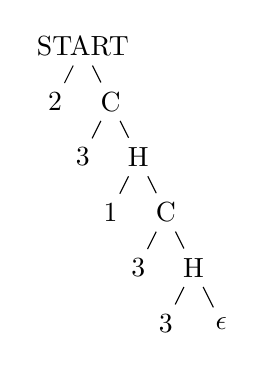
\begin{tikzpicture}[level distance=20pt,sibling distance=5pt]
\tikzstyle{level 1}=[sibling distance=20pt]
\node {START}
    child {node {2}}
    child {node {C}
        child {node {3}}
        child {node {H}
            child {node {1}}
            child {node {C}
                child {node {3}}
                child {node {H}
                    child {node {3}}
                    child {node {$\epsilon$}}
                }
            }
        }
    };
\end{tikzpicture}
&
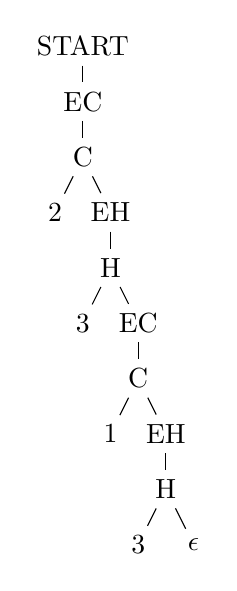
\begin{tikzpicture}[level distance=20pt,sibling distance=5pt]
\tikzstyle{level 1}=[sibling distance=20pt]
\node {START}
    child {node {EC}
        child {node {C}
            child {node {2}}
            child {node {EH}
                child {node {H}
                    child {node {3}}
                    child {node {EC}
                        child {node {C}
                            child {node {1}}
                            child {node {EH}
                                child {node {H}
                                    child {node {3}}
                                    child {node {$\epsilon$}}
                                }
                            }
                        }
                    }
                }
            }
        }
    };
\end{tikzpicture}
\end{tabular}
\end{center}
\qquad\qquad\qquad\qquad\qquad\qquad\qquad\qquad\qquad\qquad EC = "emit from cold"\\
\qquad\qquad\qquad\qquad\qquad\qquad\qquad\qquad\qquad\qquad EH = "emit from hot"
\vspace{0.3cm}


In the tree on the left, what is the meaning of an H constituent? What is the probability of the rule H $\to$ 1 C? How about the probability of H $\to \epsilon$? An equivalent approach uses a grammar that instead produces the slightly more complicated parse on the right; why might one prefer that approach?
\end{enumerate}
\end{enumerate}
\section{Building an HMM}
Make a bigram Viterbi tagger called \texttt{tag.py} that can be trained and run on the semi-supervised English data in the \texttt{data/} subdirectory. Follow the design described in the reading handout.
\marginpar{\tiny \textcircled{\tiny 2}}
Starter code and detailed \textsc{instructions} are given in the \texttt{code/} subdirectory.\footnote{If you adopt the starter code for \texttt{tag.py}, then your work will be in \texttt{hmm.py}, which it imports.} These walk you through a simple, reasonable path for building up your HMM tagger, partly using some pieces we've implemented for you, and checking your work against the ice cream spreadsheet from class. Hand in answers to the following questions:
\begin{enumerate}
\marginpar{\tiny \textcircled{\tiny 3}}
    \item[(a)] Why does Algorithm 1 initialize $\alpha_{\text{BOS}}(0)$ to 1, and Algorithm 4 initialize $\beta_{\text{EOS}}(n + 1)$ to 1?
\marginpar{\tiny \textcircled{\tiny 4}}
    \item[(b)] If you train on a \texttt{sup} file and then evaluate on a held-out \texttt{raw} file, you'll get lower perplexity than if you evaluate on a held-out \texttt{dev} file. Why is that? Which perplexity do you think is more important and why?
\marginpar{\tiny \textcircled{\tiny 5}}
    \item[(c)] V includes the word types from \texttt{sup} and \texttt{raw} (plus oov). Why not from \texttt{dev} as well?
\marginpar{\tiny \textcircled{\tiny 6}}
    \item[(d)] Did the iterations of semi-supervised training help or hurt overall tagging accuracy? How about tagging accuracy on known, seen, and novel words (respectively)?
    \item[(e)] Explain in a few clear sentences why the semi-supervised approach might sometimes help.
\end{enumerate}
\vfill
\centerline{3}

\newpage
\marginpar{\tiny \textcircled{\tiny 7}}
How does it get additional value out of the \texttt{enraw} file?\\
(Extra credit: You could investigate this empirically. For example, add some code to compare two models on a development corpus, printing out tag tokens that were incorrect under the first model but were fixed in the second model. In principle, you could even try to automatically trace what was responsible for the fix. That is, how that the good transitions/emissions are winning over the bad ones, which tokens in \texttt{enraw} contributed the fractional counts to make that happen?)
\begin{enumerate}
\marginpar{\tiny \textcircled{\tiny 8}}
    \item[(f)] Suggest at least two reasons to explain why the semi-supervised approach didn't always help.
\marginpar{\tiny \textcircled{\tiny 9}}
    \item[(g)] How does your bigram HMM tagger compare to a baseline unigram HMM tagger (see reading section G.3)? Consider both accuracy and cross-entropy. Does it matter whether you use \texttt{enraw}?
\marginpar{\tiny \textcircled{\tiny 10}}
    \item[(h)] Extra credit: Experiment with different training strategies for using \texttt{enraw}. For example, you could train on \texttt{enraw} alone, or a combined corpus of \texttt{ensup+enraw}, or \texttt{ensup+ensup+ensup+enraw} (so that the supervised data is weighted more heavily). And you could do staged training where you do additional training on \texttt{ensup} before or after this. What seems to work? Why?
\end{enumerate}
\section{Extra credit: Open-Ended Improvements}
Optionally implement an \texttt{--awesome} flag in \texttt{tag.py} that improves your cross-entropy or accuracy (on held-out data).

Your improvement should demonstrate intellectual engagement with the problem of how to improve your tagging accuracy or speed. It doesn't have to be complicated, but a one-line change is not enough by itself. More successful or interesting solutions will get more credit.

A good starting point is to study the output on the English data. As a previous question noted, our basic tagging architecture seems to get a lot of known words wrong. Think about why it might incorrectly tag a certain word as a determiner, even though that word only appeared as a noun in training data.

With this in mind, here are some things you might try:
\begin{itemize}
    \item Posterior decoding, as discussed in \textsc{instructions} and reading section D as an alternative to Viterbi tagging. (You can add this as an option for the \texttt{--loss} argument, rather than using \texttt{--awesome}.)
    
    \item Some other type of smoothing at the M-step. In choosing one, you should consider that for our particular application of HMMs—natural language part-of-speech tagging—the emission matrix $B$ is sparse. Most words have only a few possible tags. Thus, many entries in $B$ are zero (or at least very small). Perhaps you want to encourage a sparse transition matrix. For example, are there smoothing methods that pick up on the fact that some tags like D and P are closed-class tags that only allow a small set of words? Can you come up with one?
    
    \item Use hard constraints: a word that is known from supervised training data can only be tagged
\end{itemize}
\vfill
\centerline{4}

\newpage
with one of its \emph{supervised} tags.\footnote{In other words, set $\tau_j$ to a restricted set of tags that depends on $w_j$. This can be made reasonably fast by zeroing out some of the $B$ parameters.} You could choose to impose this restriction only when tagging the evaluation data (decoding), or during training as well.
\begin{itemize}
    \item Use a higher-order HMM, e.g., trigram transition probabilities instead of bigrams.
    \item Anything else you can think of!
\end{itemize}
\marginpar{\tiny \textcircled{\tiny 11}}
Discuss what you did and what you learned.

Your tagger might still fall short of the state-of-the-art 97\% for English tagging—even though the reduced tagset in Figure 2 of the reading means that you're solving an \emph{easier} problem than the state-of-the-art taggers. Why? Because you only have 100,000 words of training data (together with embeddings).

As a warning, too much experimentation with the dev data may lead to overfitting. Thus, you might consider splitting the dev data into two parts, holding some of it out to check that your final system actually works on a new dataset.
\section{Conditional Random Field Tagger}
Finally, add a simple CRF tagger to your codebase, again following the \textsc{instructions} file.

You'll use only transition and emission features. As explained in reading section E.3, this is basically equivalent to a discriminatively trained HMM—although the parameterization and training algorithm happen to be different, the main difference is that you'll be maximizing the \emph{conditional} likelihood.
\begin{enumerate}
\marginpar{\tiny \textcircled{\tiny 12}}
    \item[(a)] Compare the CRF to the HMM, training on \texttt{ensup} and evaluating on \texttt{endev}. Run a few experiments to compare them under different conditions (hyperparameters, unigram mode, features from etc.) and using different metrics (cross-entropy, accuracy). Look at the output if possible. What did you learn?
\marginpar{\tiny \textcircled{\tiny 13}}
    \item[(b)] What happens when you include \texttt{enraw} in the training data for your CRF? Explain.
\end{enumerate}
In the next homework, you'll add more useful, contextual features that can make the CRF more powerful than the HMM, although learning to wield that power correctly may still be difficult with small training data.

\section{Final Question}
\marginpar{\tiny \textcircled{\tiny 14}}
What is the maximum amount of ice cream you have ever eaten in one day? Why? Did you get sick?

\vfill
\centerline{5}
\newpage

\setcounter{page}{1}
\renewcommand{\thepage}{R-\arabic{page}}

\begin{center}
\large
\textbf{601.465/665 --- Natural Language Processing}\\
\textbf{Reading for Homework 6: Structured Prediction}
\end{center}
\begin{center}
\normalsize
Prof. Jason Eisner --- Fall 2025
\end{center}

\vspace{0.3cm}

We don't have a required textbook for this course. Instead, handouts like this one are the main readings. This handout accompanies homework 6, which refers to it.

\section*{A\quad HMM Basics}
\subsection*{A.1\quad Notation}
In this reading handout, I'll use the following notation for hidden Markov models (HMMs). You might want to use the same notation in your program.

\begin{itemize}
    \item A sentence is a word sequence $w_1, \ldots, w_n$. We also define $w_0 = \text{BOSW}$ and $w_{n+1} = \text{EOSW}$. The W is for ‘word’.
    \item The corresponding tags are $t_1, \ldots, t_n$. We also define $t_0 = \text{BOS}$ and $t_{n+1} = \text{EOS}$.
    \item We sometimes write the $i$\textsuperscript{th} tagged word as $w_i/t_i$, for example in the data files.
    \item I'll use “A” to indicate tag-to-tag \textit{transition} probabilities, as in $p_A(t_i \mid t_{i-1})$.
    \item I'll use “B” to indicate tag-to-word \textit{emission} probabilities, as in $p_B(w_i \mid t_i)$.
    \item It is sometimes convenient to put these probabilities into matrices. Suppose we have integerized the tag types. Then let the \textbf{transition matrix A} be a square matrix defined by $A_{st} = p_A(t \mid s)$. Notice that row $s$ sums to 1: it gives a probability distribution over the tags $t$ that might follow tag $s$.
    \item Suppose we have also integerized the word types. Then let the \textbf{emission matrix B} be a wide rectangular matrix defined by $B_{tw} = p_B(w \mid t)$, so row $t$ gives a probability distribution over the words $w$ that might be emitted by tag $t$. Usually this $k \times V$ matrix is wider than it is tall, since the vocabulary ($V$ words) is much larger than the tagset ($k$ tags).
\end{itemize}

\subsection*{A.2\quad Probability Model}
Now, given a tagged sentence
\[ w_1/t_1 \, w_2/t_2 \ldots w_n/t_n, \]
the probability of generating it (according to the hidden Markov model) is
\begin{equation}
    p(\mathbf{t}, \mathbf{w}) = \left(\prod_{i=1}^{n+1} p_A(t_i | t_{i-1})\right) \left(\prod_{i=1}^{n} p_B(w_i | t_i)\right)
\end{equation}

\vfill
\centerline{R-1}
\newpage
\begin{algorithm}
\caption{The forward algorithm. \textbf{w} is the input sentence, and $\boldsymbol{\tau}$ is a sequence of sets of tags. For each $j \in [1, n]$, $\tau_j$ denotes the set of possible tags for $w_j$. The algorithm returns $\sum_{\mathbf{t}: (\forall j)t_j \in \tau_j} p(\mathbf{t}, \mathbf{w})$. In the standard case, each $\tau_j$ is the set of all $k$ tags, and then the algorithm returns $p(\mathbf{w})$ (equation (3)). But it can also be made to return $Z=p(\mathbf{t}, \mathbf{w})$ (equation (1)) by taking each $\tau_j = \{t_j\}$. In general, it returns the likelihood when we observe the words \textbf{w} and we also observe the fact that each $t_j$ falls in $\tau_j$; this sums over all tagged sentences that are consistent with those observations.}
\begin{algorithmic}[1]
\Function{Forward}{$\mathbf{w}, \boldsymbol{\tau}$}
    \State $w_0 \leftarrow \text{BOSW}; \tau_0 \leftarrow \{\text{BOS}\}$ \Comment{precede word/tag sequence with BOSW/BOS}
    \State $n = |\mathbf{w}|; w_{n+1} \leftarrow \text{EOSW}; \tau_{n+1} \leftarrow \{\text{EOS}\}$ \Comment{terminate word/tag sequence with EOSW/EOS}
    \State \Comment{all $\alpha$ values are initially 0}
    \State $\alpha_{\text{BOS}}(0) \leftarrow 1$ \Comment{"start" node of the graph}
    \For{$j \leftarrow 1$ to $n+1$}
        \State \Comment{note: the loops below could be replaced by more efficient tensor operations (see equation (12))}
        \For{$t_j \in \tau_j$}
            \For{$t_{j-1} \in \tau_{j-1}$} \Comment{computes equation (7)}
                \State \Comment{find total prob of prefix paths ending in $t_{j-1}t_j$; add it to total prob of prefix paths ending in $t_j$}
                \State $p \leftarrow p_A(t_j | t_{j-1}) \cdot p_B(w_j | t_j)$ \Comment{probability of the $t_{j-1} \to t_j$ arc}
                \State $\alpha_{t_j}(j) \leftarrow \alpha_{t_j}(j) + \alpha_{t_{j-1}}(j-1) \cdot p$ \Comment{extend prefix paths starting with $t_{j-1}$; keep a running total}
            \EndFor
        \EndFor
    \EndFor
    \State $Z \leftarrow \alpha_{\text{EOS}}(n+1)$ \Comment{total prob of all complete paths (from BOS,0 to EOS,n+1)}
    \State \textbf{return} Z
\EndFunction
\end{algorithmic}
\end{algorithm}

We can also write this as a product of $2n+1$ matrix entries,
\begin{equation}
    p(\mathbf{t}, \mathbf{w}) = \left(\prod_{i=1}^{n+1} A_{t_{i-1}, t_i}\right) \left(\prod_{i=1}^{n} B_{t_i, w_i}\right)
\end{equation}
where the subscripts are the integers that represent these tags and words.

The first product is the prior probability of generating the tag sequence under a bigram model, and the second product is the probability of generating the observed words once we have chosen the tags. We don't have to generate $t_0=\text{BOS}$ because it is given, just as \textsc{root} was given in homework 1 and BOSW was given in homework 3. However, just as in homework 3, we do have to generate $t_{n+1}=\text{EOS}$, in order to know when the sentence ends: the sentence length $n \geq 0$ is the first natural number such that $t_{n+1} = \text{EOS}$.

In the above equations, we omitted the trivial factors $p_B(w_0 \mid t_0) = p_B(\text{BOSW} \mid \text{BOS}) = 1$ and $p_B(w_{n+1} \mid t_{n+1}) = p_B(\text{EOSW} \mid \text{EOS}) = 1$. However, our pseudocode will include the latter factor, for convenience.

\subsection*{A.3\quad Marginal Probabilities}
The probability of generating the words \textbf{w}---marginalizing out the tag sequence that produced those words---is
\begin{equation}
    Z = p(\mathbf{w}) = \sum_{\mathbf{t}} p(\mathbf{t}, \mathbf{w}) = \sum_{t_1} \ldots \sum_{t_n} \left(\prod_{i=1}^{n+1} p_A(t_i|t_{i-1})\right) \left(\prod_{i=1}^{n} p_B(w_i|t_i)\right)
\end{equation}

\vfill
\centerline{R-2}
\newpage

where we have observed $t_0=\text{BOS}$ and $t_{n+1}=\text{EOS}$ but have to sum over all possible taggings for the $n$ positions in between. With $k$ possible tags at each position, there are $k^n$ possible taggings to sum over! Yet as we saw in lecture, this grand summation can be computed in $O(nk^2)$ time by the \textbf{forward algorithm} (Algorithm 1). Basically, the trick is that we can express (3) as
\begin{equation}
    Z = p(\mathbf{w}) = \alpha_{\text{EOS}}(n+1)
\end{equation}
if we first define $\alpha_{t_j}(j)$ for any time step $j \in [1,n+1]$ and any possible tag $t_j$ just preceding that time step:
\begin{equation}
\alpha_{t_j}(j) \stackrel{\text{def}}{=} \sum_{t_1} \ldots \sum_{t_{j-1}} \left( \prod_{i=1}^j p_A(t_i \mid t_{i-1}) \right) \left( \prod_{i=1}^j p_B(w_i \mid t_i) \right)
\end{equation}
This represents the total probability of all prefix tag sequences for $w_1, \ldots, w_j$ that end with $t_j$. For $j \geq 2$ (so there is at least one $\sum$ symbol), it can be rearranged and written as an efficient recurrence in terms of $j-1$:
\begin{align}
\alpha_{t_j}(j) &= \sum_{t_{j-1}} \left( \sum_{t_1} \ldots \sum_{t_{j-2}} \left( \prod_{i=1}^{j-1} p_A(t_i \mid t_{i-1}) \right) \left( \prod_{i=1}^{j-1} p_B(w_i \mid t_i) \right) \right) \cdot p_A(t_j \mid t_{j-1}) \cdot p_B(w_j \mid t_j) \\
&= \sum_{t_{j-1}} \alpha_{t_{j-1}}(j-1) \cdot p_A(t_j \mid t_{j-1}) \cdot p_B(w_j \mid t_j) 
\end{align}
and that formula also works for the case $j=1$ if we take as the base case
\begin{equation}
\alpha_{\text{BOS}}(0) = 1 \qquad \alpha_{t_0}(0) = 0 \text{ if } t_0 \ne \text{BOS}
\end{equation}

\subsection*{A.4\quad Matrix Formulas}
For efficiency, let's rewrite equation (7) to use vector and matrix operations. First, we switch to using the parameter matrices $A$ and $B$. (We also rename $t_{j-1}$ and $t_j$ to $s$ and $t$ for simplicity.)
\begin{equation}
\alpha_t(j) = \sum_s \alpha_s(j-1) \cdot A_{st} \cdot B_{tw_j}
\end{equation}
Since the $B$ term doesn't depend on $s$, we can write this as
\begin{equation}
\alpha_t(j) = \left( \sum_s \alpha_s(j-1) \cdot A_{st} \right) B_{tw_j}
\end{equation}
If we regard $\vec{\alpha}(j)$ and $\vec{\alpha}(j-1)$ as row vectors indexed by tags, this is
\begin{equation}
\vec{\alpha}_t(j) = (\vec{\alpha}(j-1) \cdot A)_t \cdot B_{tw_j}
\end{equation}
or, if we want to express and compute this for all $t$ at once,
\begin{equation}
\vec{\alpha}(j) = (\vec{\alpha}(j-1) \cdot A) \odot \vec{B}_{.w_j}
\end{equation}
where $\vec{B}_{.w_j}$ denotes column $w_j$ of B, and the $\odot$ operator performs elementwise multiplication of two vectors (that is, if $\vec{c} = \vec{a} \odot \vec{b}$, then $c_t = a_t \cdot b_t$ for each $t$).\footnote{Can't we somehow just express equation (9) as a matrix multiplication? Yes, if we first define a new matrix. For any word type $w$, define the \textbf{observable operator} $P(w)$ to be the square matrix whose entries are given by}

\vfill
\centerline{R-3}
\newpage
$P(w)_{st} = A_{st} B_{tw}$. This is basically a copy of A, but where each column $t$ has been reweighted by tag $t$'s probability of emitting word $w$. In the ``trellis graph'' whose paths correspond to possible taggings, the $k \times k$ matrix $P(w_j)$ gives the weights of the $k^2$ arcs from time $j-1$ to time $j$. Now we can rewrite equation (9) as $\vec{\alpha}(j) = \vec{\alpha}(j-1)P(w_j)$. In other words, when we observe the word token $w_j$, we update the $\vec{\alpha}$ vector by multiplying it by $w_j$'s observable operator---that is, we update it by a linear transformation.

As the forward algorithm is basically just a sequence of $n+1$ such updates, we get $p(\mathbf{w}) = (\vec{\alpha}(0)P(w_1) \cdot P(w_2) \cdots P(w_n)P(w_{n+1}))_{\text{EOS}}$, or less efficiently, $p(\mathbf{w}) = (P(w_1) \cdot P(w_2) \cdots P(w_n)P(w_{n+1}))_{\text{BOS,EOS}}$, which represents the total weight of all paths of length $n+1$ from (BOS,0) to (EOS,n+1) in the trellis graph.

However, that's probably not the best way to implement it unless you have space to precompute and store the matrices $P(w)$ for all $w$. The reason is that each time you construct a copy of $P(w_j)$ from $A$ and $B$, you have to scale each column of $A$. Fewer multiplications are used by equation (12), which computes the row vector $\vec{\alpha}(j-1) \cdot A$ first and then scales each element of that row vector (faster than scaling a whole column).

\vspace{1cm}
\begin{algorithm}
\caption{The Viterbi algorithm, which finds $\text{argmax}_{\mathbf{t}: (\forall j)t_j \in \tau_j} p(\mathbf{t},\mathbf{w})$. Compare Algorithm 1.}
\begin{algorithmic}[1]
\Function{Viterbi}{$\mathbf{w}, \boldsymbol{\tau}$}
    \State $w_0 \leftarrow \text{BOSW}; \tau_0 \leftarrow \{\text{BOS}\}$ \Comment{precede word/tag sequence with BOSW/BOS}
    \State $n = |\mathbf{w}|; w_{n+1} \leftarrow \text{EOSW}; \tau_{n+1} \leftarrow \{\text{EOS}\}$ \Comment{terminate word/tag sequence with EOSW/EOS}
    \State \Comment{all $\hat{\alpha}$ values are initially 0 (or $-\infty$), and all backpointers are initially None}
    \State $\hat{\alpha}_{\text{BOS}}(0) \leftarrow 1$ \Comment{"start" node of the graph}
    \For{$j \leftarrow 1$ to $n+1$}
        \For{$t_j \in \tau_j$}
            \For{$t_{j-1} \in \tau_{j-1}$}
                \State $p \leftarrow p_A(t_j \mid t_{j-1}) \cdot p_B(w_j \mid t_j)$ \Comment{probability of the $t_{j-1} \to t_j$ arc}
                \If{$\hat{\alpha}_{t_j}(j) < \hat{\alpha}_{t_{j-1}}(j-1) \cdot p$} \Comment{keep a running maximum}
                    \State $\hat{\alpha}_{t_j}(j) \leftarrow \hat{\alpha}_{t_{j-1}}(j-1) \cdot p$ \Comment{increase the maximum}
                    \State $\text{backpointer}_{t_j}(j) \leftarrow t_{j-1}$ \Comment{and remember who provided the new maximum}
                \EndIf
            \EndFor
        \EndFor
    \EndFor
    \State \Comment{follow backpointers to find the best tag sequence that ends at the final state (EOS at time n+1)}
    \State $t_{n+1} \leftarrow \text{EOS}$
    \For{$j \leftarrow n+1$ downto 1}
        \State $t_{j-1} \leftarrow \text{backpointer}_{t_j}(j)$
    \EndFor
    \State \textbf{return} $\mathbf{t}$
\EndFunction
\end{algorithmic}
\end{algorithm}


\subsection*{A.5\quad The Viterbi Algorithm}
Algorithm 2 famously finds the most probable tagging of $\mathbf{w}$. Where the forward algorithm uses the semiring $(\oplus, \otimes) = (+, \times)$ to find the \textit{total} probability of all taggings, the Viterbi algorithm uses $(\oplus, \otimes) = (\max, \times)$ to find the \textit{maximum} probability of all taggings. To avoid confusion, we refer to this as $\hat{\alpha}$ rather than $\alpha$. It then follows backpointers to extract the argmax---that is, the tagging that achieves this maximum.

If you want to use tensor operations instead of nested loops to compute the $\hat{\alpha}$ probabilities at position $j$, try to express equation (12) in PyTorch where you express matrix multiplication without using the $\odot$ operator, instead using $*$ and \texttt{sum}. Then for Viterbi, replace \texttt{sum} with \texttt{max} (and figure out how to use \texttt{argmax} for the backpointers). Hint: The $*$ operation is \textbf{broadcastable}.

\vfill
\centerline{R-4}
\newpage

\section*{B\quad Training HMMs\protect\footnotemark}
\footnotetext{The training methods discussed in this section are much more general than just HMMs. Very similar methods apply to PCFGs, for example. They also apply to lots of other models. One nice thing about HMMs (and PCFGs) is that the probability Z of generating the observed data can be computed efficiently, by the forward (or inside) algorithm. But the methods can be used even for models where we only have slow or approximate methods for computing Z.}
\subsection*{B.1\quad Maximum Likelihood Estimation}
Let's model sentences as being generated independently of one another---all by the same HMM with parameters $A, B$. Then the probability of generating an observed sequence of sentences $\mathbf{w}_1, \mathbf{w}_2, \ldots$ is given by $\prod_m p(\mathbf{w}_m)$. This is known as the \textbf{likelihood} of the parameters $A, B$ (given this dataset). To estimate the parameters of a model, a pretty good estimation procedure (with a lot of theoretical justification) is to maximize their likelihood, or equivalently their log-likelihood:
\begin{equation}
\mathcal{L}(A, B) \stackrel{\text{def}}{=} \sum_m \log p(\mathbf{w}_m) \underset{\text{given by the sum (3)}}{\vphantom{\sum_m}}
\end{equation}
But it's wise to add a regularization term to this objective, to resist overfitting to the training data. The scale of this regularization term is, as usual, a hyperparameter $C$ that you can tune on dev data.
\begin{equation}
\underset{A, B}{\text{argmax}} \, \mathcal{L}(A, B) - C \cdot R(A, B)
\end{equation}
Above, I assumed the unsupervised setting, where you observed a sequence of untagged sentences $\mathbf{w}_1, \mathbf{w}_2, \ldots$. But what if you observed something else? In general, the likelihood of the parameters is defined as the probability of generating \textit{all the observed data} from those parameters.\footnotemark[\value{footnote}] \footnotetext{Here's a \href{https://en.wikipedia.org/wiki/Likelihood_function}{quick explanation} of what "likelihood" means in general.} So when you observe more (or less) data, you'll have to revise the definition (13) of $\mathcal{L}(A,B)$. Examples:\footnotemark[\value{footnote}] \footnotetext{An alternative is to "go full Bayesian" and get a posterior distribution over the parameters, rather than just picking one value for the parameters.}
\begin{itemize}
    \item If you have more sentences in your training corpus, then equation (13) will have more summands.
    \item If for a particular observed sentence $\mathbf{w}_m$ you also observe the tags $\mathbf{t}_m$, then you should replace $p(\mathbf{w}_m)$ with $p(\mathbf{t}_m, \mathbf{w}_m)$ in equation (13). That is, use equation (1) instead of equation (3). The probability $p(\mathbf{t}_m, \mathbf{w}_m)$ can be regarded as still summing over all the tag sequences that are consistent with the observations: but now we have enough observations that there is only one such tag sequence, so $p(\mathbf{t}_m, \mathbf{w}_m)$ is the only summand.
    \item As an advanced case, if you observe $\mathbf{w}_m$ and \textit{part} of $\mathbf{t}_m$, then you should modify equation (3) to marginalize over only the unobserved tags. For example, if you observe that $t_3 = \text{NOUN}$, then just take $t_3 = \text{NOUN}$ in the formula and remove the summation $\sum_{t_3}$ over all possible values of $t_3$. Our Algorithm 1 actually handles this case.
\end{itemize}

\subsection*{B.2\quad Discussion: Supervised, Unsupervised, and Semi-Supervised Learning}
For the \textbf{tagging task}, we are interested in learning the mapping $\mathbf{w} \to \mathbf{t}$ from a sentence to its tagging. (This is just an example of the common machine learning problem of learning an $x \to y$ mapping.) But what kind of observed data do we learn from?

\vfill
\centerline{R-5}
\newpage

\paragraph{Supervised learning.} If we observe the tags for all sentences, then we have a \textit{supervised learning} problem. In that case, you already know how to estimate the probabilities $p_A(t \mid t_{\text{prev}})$ and $p_B(w \mid t)$. Specifically, if you have a small number of probabilities to estimate, then you can just use the relative frequencies of the different transitions and emissions (see equation (17) below). This turns out to be equivalent to maximizing the log-likelihood.

If you have a larger vocabulary, then you should probably do something to avoid overfitting, for example:
\begin{itemize}
    \item smooth the counts (see reading section B.3 below)
    \item maximize the regularized log-likelihood (see equation (14) above)
    \item use a model of $p_B(w \mid t)$ that has fewer parameters (see reading section H.1 on the next homework)
\end{itemize}

\paragraph{Unsupervised learning.} The name ``hidden Markov model'' is properly used for the case where we don't observe the tags. Although the tags are governed by a Markov model (bigram model), they are \textit{hidden} (or \textit{unobserved} or \textit{missing}). The log-likelihood in equation (13) is sometimes called the \textit{incomplete-data log-likelihood} for this reason.

There are different reasons we might want to estimate an HMM. If you're using the HMM for language modeling, then the tags $\mathbf{t}$ are \textit{latent random variables}---unseen forces that we posit to help explain the observed data $\mathbf{w}$. In that case, we don't actually care about which tags are used, only that they are helpful in modeling $p(\mathbf{w})$.

But if we are actually going to evaluate on the tagging task, then this is an \textit{unsupervised learning} problem. And it's hard! We want to predict the correct tags despite never having seen any tags in training data.

\paragraph{Semi-supervised learning.} Seeing even \textit{some} of the tags makes the unsupervised problem easier. It is then called semi-supervised. For one thing, we might observe in the tagged sentences that \textit{the} usually gets tagged as \texttt{Det} and \textit{caviar} usually gets tagged as \texttt{Noun}, rather than vice-versa. (The purely unsupervised learning problem has no information to break this tie---swapping the names \texttt{Det} and \texttt{Noun} through the model would not change its likelihood function.)

How does the unsupervised data help? Even if a semi-supervised learner never observes \texttt{caviar/Noun} in the tagged sentences, it might be able to guess this tag in an untagged sentence that contains \textit{the caviar with}. It knows from the tagged sentences that \texttt{the/Det} and \texttt{with/Prep} are good guesses for those frequent words. And then it will want to guess \texttt{caviar/Noun} in between, because it knows from other tagged sentences that \texttt{Det Noun} and \texttt{Noun Prep} are common bigrams.

In other words, the highest-probability paths that explain the untagged sentence will tag this token of \textit{caviar} as \texttt{Noun}. As a result, we can best increase the likelihood by adjusting the parameters to increase $p_B(\text{caviar} \mid \text{Noun})$. That will help tag \textit{caviar} correctly in test data.\footnote{In the EM algorithm (reading sections B.4--B.5 below), the E step guesses the \texttt{Noun} tag, so the M step gets a fractional observation of \texttt{Noun} emitting \textit{caviar}, which will increase $p_B(\text{caviar} \mid \text{Noun})$. However, any other way of increasing the likelihood in reading section B.1, such as gradient ascent (reading section B.3 below), will also have this effect.}

\textbf{Unsupervised and semi-supervised learning are finicky.} As mentioned in class, \href{http://www.aclweb.org/anthology/C94-1020}{Merialdo (1994)} famously published this troubling finding:\footnote{He used unsmoothed EM to train a trigram HMM tagger, without regularization, using about a million words of newspaper text with varying amounts of supervision. The tagset had 76 different tags, corresponding to the}
\vfill
\centerline{R-6}

\newpage
\begin{figure}[h]
\centering
\includegraphics[width=0.9\textwidth]{merialdo_plot.png}
\caption{Reproduced from Merialdo (1994). Maximum-likelihood training on the unsupervised corpus from various initial points. Top line initializes with 100 supervised examples, bottom line with all 40,000 supervised examples.}
\label{fig:merialdo}
\end{figure}

Experiments show that the best training is obtained by using as much tagged text as possible. They also show that [unsupervised] maximum likelihood training, the procedure that is routinely used to estimate HMM parameters from training data, will not necessarily improve the tagging accuracy. In fact, it will generally degrade this accuracy, except when only a limited amount of hand-tagged text is available.

\vspace{0.3cm}
Increasing the log-likelihood (13) does get a better model in some sense. Certainly it improves the log-probability of the \textit{training} data---by definition. Hopefully, it will also improve the log-probability of the \textit{dev} and \textit{test} data (the cross-entropy); if not, you're overfitting to the training data and you should add a regularizer to the objective. But, as mentioned in class, there is no guarantee that it will increase the \textit{accuracy} of any tagger (reading section A.5 or reading section D). As we saw in an earlier homework, cross-entropy and accuracy are different measures.

Figure 1 is copied from Merialdo's paper. He first did supervised training on a subset of the data, then fine-tuned this with fully unsupervised training on all of the data. As you can see, when he started with a bad tagger trained on only 100 supervised sentences, its accuracy did improve for the first 3 iterations of semi-supervised training (presumably as it learned new words like \textit{caviar} from context), but then started to get worse. And if he started with any more accurate tagger, only the first 0 or 1 iterations helped! By 2 or 3 iterations, he was worse off than where he started.

The problem is that the accuracy measure demands particular “correct” tags. But the log-likelihood objective (13) doesn't actually care what tags are used on an unsupervised sentence, as long as they help to explain its words. The tagging scheme that does that best might not match
\vfill
preterminals of a syntactic treebank.
\centerline{R-7}

\newpage
the tagging scheme in the supervised data. The supervised tags were specifically chosen to be coarse-grained preterminals. Yet to predict the words of the unsupervised sentences, it might be \emph{more useful} to keep track of whether there was a recent transitive verb, or whether the sentence is about politics! So unsupervised learning might repurpose a tag like \texttt{F} (foreign word) to mean something else. We already saw this in class with the ice cream spreadsheet, where EM training sometimes used the \texttt{H} tag to mean something other than the intended ``hot day.''

To stick to the intended use of the tags, it might help to take supervision into account in a more serious way than Merialdo did. His objective function completely ignored the supervised data---it was the wholly unsupervised log-likelihood objective (13). This ignores the supervised data, which would have been \emph{wholly irrelevant} if he'd used a magical optimizer that found the global maximum of (13). The supervised data only influenced his tagger because his optimization algorithm (EM) got stuck in a local maximum near his supervised initialization point. So we could change the objective function to consider the supervised data explicitly. Some possibilities:
\begin{itemize}
    \item If $\theta_{\text{sup}}$ is the parameters of the initial supervised model, you could modify the unsupervised objective equation (13) by adding a regularizer $||\theta - \theta_{\text{sup}}||^2$ to your unsupervised objective. This is basically doing L2 regularization on the \textit{change} in the parameters, to discourage them from forgetting the initializer.
    
    \item You could use a semi-supervised log-likelihood objective: the sum of $\log p(\mathbf{t}, \mathbf{w})$ on the supervised sentences and $\log p(\mathbf{w})$ on the unsupervised sentences. Then you still get some guidance from the supervised data. \textbf{You'll try this version in the homework.}
    
    \item Unfortunately, if you have 100 supervised sentences and 39,900 unsupervised sentences, like Merialdo, then the objective function will be dominated by the untrustworthy guessed tags. The good tags will have very little influence. So you could try to fix this by placing more weight on the supervised sentences.\footnote{One quick method is to include many copies of them in the semi-supervised training corpus.} This weight is a hyperparameter.
    
    \item Rather than set a weight, you could try to maximize the unsupervised objective \emph{subject to the constraint} that the tagging of the 100 supervised sentences stays \emph{as good} as it was in the supervised model.\footnote{This could mean that the Viterbi tagging doesn't get worse than it was in the supervised model, or that the posterior tagging doesn't get worse, or that $\log p(\mathbf{t} \mid \mathbf{w})$ doesn't decrease (where $\mathbf{t}$ is the supervised tagging).} However, this requires constrained optimization techniques.
    
    \item Use a semi-supervised \textit{discriminative} objective: the sum of $\log p(\mathbf{t} \mid \mathbf{w})$ on the supervised sentences (see equation (24)) and $\log p(\mathbf{w})$ on the unsupervised sentences.
\end{itemize}
Again, you can place less weight on the unsupervised term. In effect, the supervised term $\sum_m \log p(\mathbf{t}_m \mid \mathbf{w}_m)$ term more or less captures your real objective, which is to do a good job of tagging. The unsupervised term $\log p(\mathbf{w})$ acts as a “multi-task regularizer” that encourages the parameters to also be good at predicting word sequences. The weight of the regularizer is a hyperparameter, as usual.
\vfill
You are welcome to try any of the ideas above for extra credit.
This last one would actually be pretty easy to try, using one Lagrange multiplier per sentence. In fact, it's similar to the method below that puts $\log p(\mathbf{t} \mid \mathbf{w})$ directly into the objective. The difference is that now the weight of that term will vary by sentence: it's a Lagrange multiplier that will \emph{automatically} be increased as much as necessary in order to get $\log p(\mathbf{t}|\mathbf{w})$ as high as it was in the supervised model. No hyperparameter is needed.
\centerline{R-8}

\newpage

\subsection*{B.3 Procedures for Optimizing $A, B$}
\paragraph{Relative frequency estimation.} If you have fully supervised data, then the log-likelihood is
\begin{align}
\mathcal{L}(A,B) & \stackrel{\text{def}}{=} \sum_m \log p(\mathbf{t}_m, \mathbf{w}_m) \underset{\text{given by (1)}}{\vphantom{\sum}} \\
& = \sum_m \left( \sum_{i=1}^{n+1} \log p_A(t_i|t_{i-1}) \right) + \left( \sum_{i=1}^{n} \log p_B(w_i|t_i) \right)
\end{align}
and as mentioned above, this is trivial to optimize! The log-likelihood function is concave, and the globally optimal values are just count ratios, as on the language modeling homework:
\begin{equation}
p_A(t_i|t_{i-1}) = \frac{c(t_{i-1}, t_i)}{c(t_{i-1})} \qquad p_B(w_i|t_i) = \frac{c(t_i, w_i)}{c(t_i)}
\end{equation}
To resist overfitting to the training data, you can use add-$\lambda$ smoothing or another smoothing technique, as noted above.

\paragraph{Gradient ascent.} When some or all tags are unobserved, the log-likelihood or regularized log-likelihood function from reading section B.1 can have multiple local optima. The global optimum is now very hard to find. But we can at least try to improve the function up to a local optimum.

How should we do that? Gradient ascent is an obvious direct approach. You already know how to do SGD from the language modeling homework. We'll switch to SGD when we reach CRFs (question 4 and reading section E), and we'll continue using SGD on the next homework.

\paragraph{The EM algorithm.} However, first we'll explore maximizing log-likelihood by Expectation-Maximization (EM), as illustrated in class with the ice cream spreadsheet. EM is an attractive method that is often faster. The M step often makes a big change to the parameters in place of taking many little steps as in gradient ascent. It's not even necessary to choose a stepsize! The EM method is developed in the following sections, without proofs.

\subsection*{B.4\quad Monte Carlo Expectation-Maximization (MCEM)}
The incomplete-data likelihood (13) \textit{sums} over all possible taggings for each sentence. A variant approach is to \textit{impute} each sentence's tagging, i.e., guess what it might be. This gives us a “supervised'' version of the corpus, on which we can train our parameters to maximize the \textit{complete-data} likelihood. In other words, we use imputation to convert the unsupervised learning problem into a supervised learning problem that we can solve with equation (17)!

How does this work? For each sentence $\mathbf{w}_m$ in the training corpus, we randomly sample a guess $\hat{\mathbf{t}}_m$ of its tag sequence. The guess $\hat{\mathbf{t}}_m$ should be sampled from the posterior distribution $p(\mathbf{t} \mid \mathbf{w}_m)$ defined by the \textit{current} model parameters. In other words, we will probably sample a tagging that the model thinks has a high chance of being correct.

If we pretend that $\hat{\mathbf{t}}_m$ really is correct, then $(\hat{\mathbf{t}}_m, \mathbf{w}_m)$ is a \textit{supervised} version of the sentence. However, of course it's just a guess---the true tags $\mathbf{t}_m$ are missing (or ``hidden'') and we have no way to know for sure what they were. $\hat{\mathbf{t}}_m$ may not even be a good guess, because the current model parameters aren't correct. But we can iterate the procedure, which will work in some sense.

\vfill
\centerline{R-9}

\newpage

We use the current parameters to make the guesses (the \textbf{Monte Carlo E step}). Then we do supervised training via (17) to re-estimate the parameters (the \textbf{M step}). So our next E step will have better guesses, and so on. This iterative procedure is known as the \textbf{Monte Carlo EM algorithm (MCEM)}.\footnote{`Monte Carlo'' algorithms are algorithms that use randomness. The name was originally a military code name, referring to a casino in Monaco---casinos also use randomness.}

\paragraph{Correctness.} Does this algorithm maximize the likelihood? A first problem is that it might not even converge. Even if we were to reach the maximum-likelihood parameters, we wouldn't stay there, because on the next iteration we'd make different random guesses, so equation (17) would change. In general, our estimated probabilities (17) will keep bouncing around due to the randomness.

However, the law of large numbers implies that if the total number of sentences $M$ is large, the count ratios in (17) will usually be pretty close to their theoretical expectation. If $M$ is small, you can get the same effect by sampling $S$ different taggings per sentence, increasing the number of randomly tagged sentences to $SM$. (This is known as ``multiple imputation'' and is widely used in statistics to deal with missing data.) As $S \to \infty$, the counts $c(\cdots)$ get large and the variance in the estimated probabilities (17) shtrinks to 0. Thus, one way to gradually remove the randomness is to \textit{increase} $S$ on each iteration. MCEM then indeed converges to a (local) maximum of log likelihood.\footnote{An alternative way to get MCEM to converge is to replace the M steps with SGD steps. At each step, sample a mini-batch of sentences $\mathbf{w}_m$ from the training corpus, then impute tags $\hat{\mathbf{t}}_m$ for each sentence in the mini-batch, and then take a gradient step on these supervised sentences to try to improve the mini-batch log-likelihood $\sum_m \log(\hat{\mathbf{t}}_m, \mathbf{w}_m)$. There is already randomness in the choice of mini-batch, so the additional randomness in the imputation is not a problem---SGD can still converge due to the decreasing stepsize over time. Recall that the stochastic gradient in SGD only has to be correct in expectation. In our setting, it's not actually true that the expectation of $\nabla \log p(\hat{\mathbf{t}}_m, \mathbf{w}_m)$ is $\nabla \log p(\mathbf{w}_m)$. But even so, this procedure also turns out to be correct; it again converges to a (local) maximum of log-likelihood.}

\paragraph{Efficiency.} MCEM is easy to understand: it simply converts semi-supervised learning to supervised learning by multiple imputation. It is practically useful in advanced machine learning models where the summation in equation (13) is computationally expensive, but where imputation is cheaper. That is, it's useful when there's an efficient procedure\footnote{Often a Markov chain Monte Carlo method such as Gibbs sampling.} for sampling the latent variable $\mathbf{t}$ from the posterior $p(\mathbf{t} \mid \mathbf{w}_m)$, either exactly or approximately.

But what is the sampling procedure for HMMs? That is, how do we draw a random tagging from the posterior distribution $p(\mathbf{t} \mid \mathbf{w}_m)$? A ``backward sampling'' algorithm is shown in Algorithm 3. It is sort of a randomized version of the Viterbi algorithm---instead of following the \textit{best} backpointers to find the \textit{most probable} tag sequence, it follows \textit{random} backpointers to find a \textit{random} tag sequence. Of course, the tag sequences aren't all equally probable! If most of the paths to Noun at token 8 come through Det at token 7, then most of $\alpha_{\text{Noun}}(8)$ will be contributed by $\alpha_{\text{Det}}(7)$, and the random $\text{backpointer}_{\text{Noun}}(8)$ will probably be Det.

This sampling procedure is efficient, but it's not \textit{more} efficient than summation. To figure out which paths contribute most, we first have to do all the work of the forward algorithm. So in the case of HMMs, sampling one tagging is not in fact more efficient than summing over all of the taggings.

\vfill
\centerline{R-10}

\newpage
\begin{algorithm}
\caption{Forward algorithm with backward sampling. This is a variant of the forward algorithm (Algorithm 1) that keeps randomized backpointers, and then follows them just as in the Viterbi algorithm (Algorithm 2).}
\begin{algorithmic}[1]
\Function{Random-Tagging}{$\mathbf{w}, \boldsymbol{\tau}$}
    \State $w_0 \leftarrow \text{BOSW}; \tau_0 \leftarrow \{\text{BOS}\}$ \Comment{precede word/tag sequence with BOSW/BOS}
    \State $n = |\mathbf{w}|; w_{n+1} \leftarrow \text{EOSW}; \tau_{n+1} \leftarrow \{\text{EOS}\}$ \Comment{terminate word/tag sequence with EOSW/EOS}
    \State \Comment{all $\alpha$ values are initially 0}
    \State $\alpha_{\text{BOS}}(0) \leftarrow 1$ \Comment{"start" node of the graph}
    \For{$j \leftarrow 1$ to $n+1$}
        \For{$t_j \in \tau_j$}
            \For{$t_{j-1} \in \tau_{j-1}$}
                \State $p \leftarrow p_A(t_j \mid t_{j-1}) \cdot p_B(w_j \mid t_j)$ \Comment{probability of the $t_{j-1} \to t_j$ arc}
                \State $\alpha_{t_j}(j) \leftarrow \alpha_{t_j}(j) + \alpha_{t_{j-1}}(j-1) \cdot p$
                \State with probability of $(\alpha_{t_{j-1}}(j-1) \cdot p) / \alpha_{t_j}(j)$ \Comment{keep a running sample}
                    \State $\text{backpointer}_{t_j}(j) \leftarrow t_{j-1}$
            \EndFor
        \EndFor
    \EndFor
    \State \Comment{follow backpointers to extract a random tag sequence that ends at the final state (EOS at time $n+1$)}
    \State $t_{n+1} \leftarrow \text{EOS}$
    \For{$j \leftarrow n+1$ downto 1}
        \State $t_{j-1} \leftarrow \text{backpointer}_{t_j}(j)$
    \EndFor
    \State \textbf{return} $\mathbf{t}$
\EndFunction
\end{algorithmic}
\end{algorithm}
Therefore, we won't ask you to use Monte Carlo EM. Instead, we'll use true EM, which uses the forward-backward algorithm. True EM is equivalent to Monte Carlo EM with $S=\infty$. This also avoids the noise from random sampling.\footnote{Again, the other option would be to simply follow the gradient of the incomplete-data log-likelihood (13), which involves a summation that can be computed by the forward algorithm.}

\subsection*{B.5\quad Expectation-Maximization (EM)}
The procedure shown on the spreadsheet in class was the classical EM procedure, which can be understood as ``MCEM without randomness.'' EM averages over all ways of guessing the tag sequence, instead of randomly sampling just one (or a finite number $S > 1$) as in MCEM.

So instead of increasing $\log p(\hat{\mathbf{t}}_m, \mathbf{w}_m)$ for a \textit{particular} (random) tag sequence $\hat{\mathbf{t}}_m$, EM increases the expected value of that quantity, namely $\mathbb{E}_{\mathbf{t} \sim p(\mathbf{t}|\mathbf{w}_m)} \log p(\mathbf{t}, \mathbf{w}_m)$. This is the behavior that multiple imputation approaches in the limit $S \to \infty$.

Traditional EM doesn't even have SGD's randomness of choosing different examples $\mathbf{w}_m$ at different steps.\footnote{Although that is a possible variant: \href{https://www.cs.cmu.edu/~percy/papers/liang-klein-nips2009.pdf}{Liang \& Klein (2009)} found that "stepwise EM" using minibatches is quite effective. Having some randomness in the objective can help jolt the optimizer out of local optima.} Rather, the M step is a "batch" procedure that tries to maximize the expected log-likelihood of the whole training corpus, i.e.,
\begin{equation}
\sum_m \sum_{\mathbf{t}} \underbrace{p(\mathbf{t} | \mathbf{w}_m)}_{\text{hold constant}} \log p(\mathbf{t}, \mathbf{w}_m)
\end{label}
\end{equation}
It's important to understand exactly what's being maximized here. The coefficients $p(\mathbf{t} | \mathbf{w}_m)$ are computed by the \textbf{E step} and are then held fixed during the \textbf{M step}. That is, the first $p$ in this

\vfill
\centerline{R-11}
\newpage

formula is a constant copy of the "current" $p$. We adjust only the second $p$ during maximization. This looks for new parameters $A,B$ that give high log-probabilities $\log p(\mathbf{t}, \mathbf{w}_m)$ to the ``currently'' probable taggings $\mathbf{t}$. Equation (18) is convex in $A, B$, so we really can globally maximize it.

Once we've maximized equation (18), we use these new parameters to make new guesses---another E step---and then do another M step, and so on. Again, this turns out to be a valid procedure for (locally) maximizing equation (13).\footnote{Why? It can be shown (via something called Jensen's inequality) that equation (18) is always $\le$ equation (13). So by finding parameters that make the lower bound (18) high, we can ensure that the log-likelihood (13) is also high. Furthermore, it can be be shown that when EM converges—meaning that two successive E steps return the same distribution $p(\mathbf{t} \mid \mathbf{w}_m)$—the two quantities are equal and both are at a local maximum. Thus, EM locally maximizes equation (13). Monte Carlo EM (reading section B.4) is essentially the stochastic version of this procedure.}

Crucially, for an HMM, we can maximize equation (18) efficiently.\footnote{For fancier models where this is not true, a useful generalization is \textbf{variational EM}. Namely, when there is no efficient way to work with $p(\mathbf{t}|\mathbf{w}_m)$ in equation (18), we can use a more tractable distribution $q_m(\mathbf{t})$ over the taggings. No matter what distribution $q_m$ we pick, we'll still get a lower bound on the log-likelihood (still by Jensen's inequality). So the variational E step tries to increase the lower bound $\sum_m \mathbb{E}_{\mathbf{t}\sim q_m(\mathbf{t})} \log p(\mathbf{t}, \mathbf{w}_m)$ by reestimating the distributions $q_m$ (while keeping them tractable), and the M step tries to increase it by reestimating the model $p$.} We don't have to iterate over all $k^n$ possible taggings for a sentence of length $n$. It turns out that to maximize equation (18) at the M step, we only need the total \textit{fractional counts} of the transitions and emissions, which we feed into equation (17).\footnote{Can you prove this? Hint: start by using equation (1) to expand the $\log p$ term in equation (18).} So that is all that the E step computes. For a given sentence, the forward-backward algorithm of Algorithm 4 computes the fractional counts in $O(nk^2)$ time via dynamic programming. We compute the total counts by running Algorithm 4 on all the sentences.\footnote{How about a matrix version? Footnote 1 noted that the forward algorithm amounted to computing a sequence of row vectors via $\vec{\alpha}(j) = \vec{\alpha}(j-1)P(w_j)$, where the base case $\vec{\alpha}(0)$ is the row vector that is one-hot at BOS. In the same way, the backward algorithm amounts to computing a sequence of column vectors via $\vec{\beta}(j-1) = P(w_j)\vec{\beta}(j)$, where the base case $\vec{\beta}(n+1)$ is the column vector that is one-hot at EOS. We obtain Z as $\alpha_{\text{EOS}}(n+1)$ or alternatively as $Z=\beta_{\text{BOS}}(0)$. The posterior distribution over the tag $T_j$ is given by the vector $\vec{\alpha}(j) \odot \vec{\beta}(j) / Z$.}

The M step is just like training on a supervised corpus. Each untagged training sentence $\mathbf{w}_m$ has given rise to lots of tagged training sentences $(\mathbf{t}, \mathbf{w}_m)$, which are all ``fractionally'' in the corpus. Our old supervised training methods work. Specifically, you can maximize equation (18) by setting the transition and emission probabilities as ratios (17) of fractional counts.

\subsection*{B.6\quad Don't Guess When You Know}
``Don't guess when you know'' is a good general principle. If there are things that \textit{can't} or \textit{must} happen, then you may as well ensure that their probabilities in your model are 0 or 1, respectively.

The relative frequency estimates (17) will actually get this right—e.g., they will assign probability 0 to something that never happened in your reconstructed supervised taggings. But what if you smooth those estimates? Smoothing tries to avoid estimating probabilities as 0. A naive implementation of add-$\lambda$ smoothing at the M step will produce estimates in (0,1) even for probabilities that you know must be 0 or 1.

It's not the end of the world if you estimate 0.00001 for something that you know is 0. But it's good software design to nail down that known 0, unless handling that special case makes the code slow or ugly. This is known as a ``structural zero'' in the model---it's part of the model's structure, not something you estimate.

In particular, we know about $p_B$:
\begin{itemize}
    \item $p_B(\text{BOSW} \mid \text{BOS}) = 1$
\end{itemize}

\vfill
\centerline{R-12}

\newpage
\begin{algorithm}[h!]
\caption{Forward-backward algorithm for computing emission counts $c(t,w)$ and expected transition counts $c(s,t)$. This algorithm increments the existing counts $c(\cdots)$ by the counts from this sentence.}
\begin{algorithmic}[1]
\Function{Forward-Backward}{$\mathbf{w}, \boldsymbol{\tau}$}
    \State run Algorithm 1 to compute the $\alpha$ values as well as $n, w_0, \tau_0, w_{n+1}, \tau_{n+1}$, and $Z$
    \State \Comment{now for the backward pass; all $\beta$ values are initially 0}
    \State $\beta_{\text{EOS}}(n+1) \leftarrow 1$
    \For{$j \leftarrow n+1$ downto 1}
        \For{$t_j \in \tau_j$}
            \State $c(t_j, w_j) \text{ += } \alpha_{t_j}(j) \cdot \beta_{t_j}(j) / Z$ \Comment{increment count by $p(T_j = t_j \mid \mathbf{w}, \boldsymbol{\tau})$}
            \For{$t_{j-1} \in \tau_{j-1}$}
                \State \Comment{find total prob of all suffix paths that start with $t_{j-1}t_j$,}
                \State \Comment{and add it to total prob of suffix paths starting with $t_{j-1}$}
                \State $p \leftarrow p_A(t_j \mid t_{j-1}) \cdot p_B(w_j \mid t_j)$ \Comment{probability of the $t_{j-1} \to t_j$ arc (same as in forward pass)}
                \State $c(t_{j-1}, t_j) \text{ += } \alpha_{t_{j-1}}(j-1) \cdot p \cdot \beta_{t_j}(j) / Z$ \Comment{increment by $p(T_{j-1} = t_{j-1}, T_j = t_j \mid \mathbf{w}, \boldsymbol{\tau})$}
                \State $\beta_{t_{j-1}}(j-1) \text{ += } p \cdot \beta_{t_j}(j)$ \Comment{left-extend suffix path starting with $t_j$; add to running total}
            \EndFor
        \EndFor
    \EndFor
    \State \textbf{assert} $\beta_{\text{BOS}}(0) = Z$ \Comment{backward algorithm computes same sum as forward}
\EndFunction
\end{algorithmic}
\end{algorithm}
\begin{itemize}
    \item $p_B(\text{BOSW} \mid t) = 0$ for $t \ne \text{BOS}$
    \item $p_B(\text{EOSW} \mid \text{EOS}) = 1$
    \item $p_B(\text{EOSW} \mid t) = 0$ for $t \ne \text{EOS}$
\end{itemize}
To avoid all of these special cases, let's just say that $B$ only provides the emission probabilities $p_B(w_j|t_j)$ for $j \in [1, n]$, so it never conditions on $t_0=\text{BOS}$ or $t_{n+1}=\text{EOS}$. In fact, equation (1) only considers those emission probabilities. (It's true that Algorithm 1 line 11 does look up $p(\text{EOSW} | \text{EOS})$, but that factor can be skipped or forced to 1 by a simple ``if'' test. There's no need to actually look it up in $B$.)

Then we don't need rows in the $B$ matrix for BOS and EOS. And we don't need columns for BOSW and EOSW---we can actually leave them out of the vocabulary. Then each row of $B$ is a probability distribution over the vocabulary and cannot give any probability to BOSW or EOSW.

You can physically omit the rows in B for BOS and EOS if you add them last to the tag integerizer; then a matrix with $k-2$ rows will have rows indexed by the other tags. Alternatively, it's okay if those tags have rows in the matrix, but they should never be accessed. Set them to 0, or to NaN so that you get an error if they are accidentally used.

We also know about $p_A$:
\begin{itemize}
    \item $p_A(\text{BOS} \mid s)=0$ for any preceding tag $s$
    \item $p_A(t \mid \text{EOS})$ doesn't matter (will not be used)
\end{itemize}
So it would be nice to omit the BOS column and the EOS row from the $A$ matrix.

The problem is that $\vec{\alpha}(j)$ should have $k$ elements—one for each tag including BOS (nonzero for $j=0$) and EOS (nonzero for $j=n+1$). So if we're going to multiply by $A$ to transform that vector (equation (12)), we need $A$ to be $k \times k$.

The best option is probably to force the \textsc{bos} column to be 0. For example, if you set the BOS column of $W^A$ to $-\infty$, then exponentiating it will give a column of zeroes in $A$. Then you can set the EOS row to be NaN.

\vfill
\centerline{R-13}
\newpage

(In Python, use \texttt{math.nan} and \texttt{-math.inf}, or \texttt{float("nan")} and \texttt{float("-inf")}).

\section*{C\quad Numerical Issues}
For long sentences or large vocabularies, the $\alpha$ and $Z$ probabilities for a sentence will be quite small. You'll need a method for preventing underflow. Here are a few options.\footnote{These methods can also help prevent \textit{overflow}. Overflow could arise during exponentiation in equation (54) or equations (31)-(45) if you have allowed the weights to get too large. However, if the weights are really large enough to cause overflow, then it probably means you've taken too large a gradient step or you haven't regularized enough.}

\subsection*{C.1\quad The Scaling Trick}
A simple, efficient, and effective option is to just scale the probabilities up when they get small. Recall our update rule (equation (12)):
\begin{equation}
\vec{\alpha}(j) \leftarrow (\vec{\alpha}(j-1) \cdot A) \odot B_{.w_j}
\end{equation}
Suppose after we compute this, we divide it by a small constant $\kappa_j$:
\begin{equation}
\vec{\alpha}(j) \leftarrow \vec{\alpha}(j)/\kappa_j
\end{equation}
Now $Z$ in Algorithm 1 will be off by a factor of $\prod_j \kappa_j$. But you can easily multiply that back in at the end of the algorithm (line 13).
\begin{equation}
Z \leftarrow \alpha_{\text{EOS}}(n+1) \cdot \prod_j \kappa_j
\end{equation}
except that to avoid underflow, you should switch to logspace:
\begin{equation}
\log Z \leftarrow \log \alpha_{\text{EOS}}(n+1) + \sum_j \log \kappa_j
\end{equation}
So you just have to keep a running total $\sum_j \log \kappa_j$ as you go. The only reason to keep this running total is to report $\log Z$ accurately so that you can watch this log-likelihood improve over time.

You could choose $\kappa_j$ to be any positive constant. It's just a bookkeeping convenience to avoid underflow. An elegant choice is $\kappa_j = \sum_t \alpha_t(j)$ because then the rescaled $\vec{\alpha}(j)$ then gives the relative probabilities of the tags (i.e., they sum to 1). Another reasonable choice would be $\kappa_j = \max_t \alpha_t(j)$, in which case the rescaled $\vec{\alpha}(j)$ will have a max value of 1.

A couple of fancy improvements you could consider:
\begin{itemize}
    \item At steps $j$ where this sum or max is not very small, you could optionally just skip the rescaling step (equivalent to taking $\kappa_j=1$). This means you only have to rescale every so often, when the probabilities are in danger of underflowing.
    \item You could ensure that $\kappa_j$ is a power of 2, which means that there are especially fast ways to multiply $\vec{\alpha}(j)$ by $\kappa_j$. (This is probably not worth it, unless you're writing low-level code, but it connects nicely to the discussion in reading section C.3 below.)
\end{itemize}
Note that this trick works for tagging specifically. How would you make it work for parsing? (The most obvious approach is wrong. I can see a solution, but it took a little thought!) The next solution is more general, but also more annoying.

\vfill
\centerline{R-14}

\newpage

\subsection*{C.2\quad Log Probabilities}
A common general trick for avoiding underflow is to store your probabilities ``in logspace'' (or equivalently, ``in the log domain''). That is, when you see something like $p=q \cdot r$, implement it as something like $lp=lq+lr$, where $lp,lq,lr$ are variables storing the logs of the probabilities. Note that $\log 0 = -\infty$. (Which is a number, not an exception. \texttt{numpy.log(0)} will indeed return the floating-point representation of $-\infty$, which can also be obtained directly by \texttt{-math.inf} or \texttt{-numpy.inf}. PyTorch behaves similarly.)

\paragraph{Addition in logspace.} The forward algorithm requires you to add probabilities, as in $p \leftarrow p+q$. But you are now storing these probabilities $p$ and $q$ as their logs, $lp$ and $lq$.

You might try to write $lp \leftarrow \log(\exp lp + \exp lq)$, but the $\exp$ operation will probably underflow and return 0---that is why you are using logs in the first place!

Instead, the function \texttt{logaddexp(lp, lq)} is available in numpy and PyTorch. It safely does the computation above. That is, it adds two values that are represented in logspace. (If you want to sum a whole sequence of values, use \texttt{logsumexp}.) How does it work?
\begin{equation}
\text{logaddexp}(x, y) \stackrel{\text{def}}{=} 
\begin{cases}
    x + \log(1+\exp(y-x)) & \text{if } y \le x \\
    y + \log(1+\exp(x-y)) & \text{otherwise}
\end{cases}
\end{equation}
You can check for yourself that this equals $\log(\exp x + \exp y)$; that the $\exp$ can't overflow (because its argument is always $\le 0$); and that you get an appropriate answer even if the $\exp$ underflows.

The sub-expression $\log(1+z)$ can be computed more quickly and accurately by the specialized function $\text{log1p}(z) = z - z^2/2 + z^3/3 - \cdots$ (Taylor series), which is usually available in the math library of your programming language (or see \url{http://www.johndcook.com/cpp_log_one_plus_x.html}). This avoids ever computing $1+z$, which would lose most of $z$'s significant digits for small $z$. Make sure to handle the special case where $p=0$ or $q=0$ (see above).

\paragraph{Tensor operations.} After you update A and B at the M step (by equation (17) or a smoothed version), you will have to take their logs to get versions $lA$ and $lB$, whose entries are log-probabilities.
Recall that equation (12) involves a product of the row vector $\vec{\alpha}(j-1)$ with the square matrix A. But if you are representing these using logspace tensors, you can't use the ordinary matrix product operator @. You need a version that uses \texttt{+} and \texttt{logsumexp} (in place of the usual \texttt{*} and \texttt{sum}). You'll have to figure out how to do this efficiently with PyTorch tensor operations. Just as in reading section A.5, a good first step is to try to implement $\odot$ using only $*$ and \texttt{sum}.

\paragraph{What kind of logs?} To simplify your code and avoid bugs, this section has recommended that you use log-probabilities rather than negative log-probabilities. Then you won't have to remember to negate the output to log or the input to exp. (The convention of negating log-probabilities helps to keep minus signs out of the \textit{printed numbers}; but when you're coding, it's safer to keep minus signs out of the \textit{formulas and code instead}.)

Similarly, I recommend that you use natural logarithms ($\log_e$) because they are simpler than $\log_2$, slightly faster, less prone to programming mistakes, and supported by library functions like \texttt{logsumexp}.
Yes, it's conventional to report $-\log_2$ probabilities, (the unit here is ``bits''). But you can store $\log_e x$ internally, and convert to bits only when and if you print it out: $-\log_2 x = -(\log_e x) / \log_e 2$.
\vfill
\centerline{R-15}

\newpage
(As it happens, you won't be required to print any log-probabilities for this homework, only perplexities: see equation (38).)

\subsection*{C.3\quad High Precision Arithmetic}
A final possibility is to use a type of number that won't underflow. 32-bit floating point numbers can get as small as $10^{-38}$, and 64-bit floating point numbers can get as small as $10^{-308}$. But there are Python libraries for high-precision arithmetic, such as \texttt{mpmath}, \texttt{bigfloat}, and \texttt{mxNumber}. These use more than 64 bits to represent a number---indeed, they can expand the size of the representation as necessary.

Recall that a floating point number stores a fixed-point mantissa together with an integer exponent which is basically the $\log_2$ of the number (rounded towards zero). So to avoid underflow, really what we want is to have a lot of bits in the exponent.

The previous alternatives can be actually thought of specialized floating-point representations\footnote{Indeed, the previous alternatives could be packaged up as numeric classes. For example, you could make a \texttt{PosNum} class that stores any positive number $p$ as $\log p$ (and perhaps stores 0 as $-\infty$), which enables it to represent very small probabilities. You'd then implement arithmetic operations such as $*,+,$ and $\max$. You'd also need a constructor that turns a nonnegative real into a \texttt{PosNum} (using log), and a method for extracting the real value of a \texttt{PosNum} (using exp).} that focus on the exponent:
\begin{itemize}
    \item In the scaling trick of reading section C.1, the running total $\sum_{i=1}^{j-1} \log \kappa_i$ can be regarded as a possibly large, possibly non-integer exponent that is shared by all of the values in $\vec{\alpha}(j)$.
    \item The logspace trick of reading section C.2 can be thought of as a numeric representation where the mantissa is 1 and the exponent is itself a floating point number (allowing it to be very large). Indeed, \texttt{logaddexp} is actually rather similar to floating-point addition.\footnote{Before adding two numbers, floating-point addition has to multiply the mantissa of the smaller number by $2^{y-x}$, where $y-x<0$ is the difference between the integer exponents. This is similar to equation (23). But in the floating-point case, multiplying the mantissa by $2^{y-x}$—which is an integer power of 2—is easily accomplished by right-shifting the bits of its binary representation.}
\end{itemize}
Using the general high-precision arithmetic libraries is probably too slow and unnecessarily precise, and won't work with PyTorch.

\section*{D\quad Posterior Decoding}
\textbf{Decoding} refers to extracting a prediction from the model. Recall that a Viterbi decoder (reading section A.5) finds the single most likely overall sequence. By contrast, a posterior decoder will separately choose the best tag at each position---the tag with highest posterior marginal probability---even if this gives an unlikely overall sequence.

In Algorithm 4, the probability that tag $T_j$ has value $t_j$ is computed at line 7 (which adds it to $c(t_j, w_j)$). The posterior marginal distribution over all possible tags at position $j$ can be found efficiently as $\vec{\alpha}(j) \odot \vec{\beta}(j)/Z$.\footnote{In the next homework, reading section K will lay out a way to compute this without implementing Algorithm 4 (the backward pass). Instead, it uses back-propagation.}

Here's an example of how posterior decoding works (repeated from the HMM slides in class). Suppose you have a 2-word string, and the HMM assigns positive probability to three different tag sequences, as shown at the left of this table:
\vfill
\centerline{R-16}

\newpage
\begin{table}[h]
\centering
\begin{tabular}{c | c c | c c c c c c}
    & & & \multicolumn{6}{c}{score if predicted sequence is ...} \\
prob & \multicolumn{2}{c|}{actual sequence} & N V & Det Adj & Det N & Det V & $\cdots$ \\
\hline
0.45 & N & V & 2 & 0 & 0 & 1 & $\cdots$ \\
0.35 & Det & Adj & 0 & 2 & 1 & 1 & $\cdots$ \\
0.2  & Det & N & 0 & 1 & 2 & 1 & $\cdots$ \\
\hline
\multicolumn{3}{c|}{expected score} & 0.9 & 0.9 & 0.75 & 1.0 & $\cdots$
\end{tabular}
\end{table}

The Viterbi decoder will return \texttt{N V} because that's the most probable tag sequence. However, the HMM itself says that this has only a 45\% chance of being correct. There are two other possible answers, as shown by the rows of the table, so \texttt{N V} might be totally wrong.

So is \texttt{N V} a good output for our system? Suppose we will be evaluated by the number of correct tags in the output. The \texttt{N V} column shows how many tags we might get right if we output \texttt{N V}: we have a 45\% chance of getting 2 tags right, but a 55\% chance of getting 0 tags right, so \textit{on average} we expect to get only 0.9 tags right. The \texttt{Det Adj} or \texttt{Det N} columns show how many tags we'd expect to get right if we predicted those sequences instead.

It's not hard to see that with this evaluation setup, the best way to maximize our score is to separately predict the most likely tag at every position. We predict $t_1 = \text{Det}$ because that has a 0.55 chance of being right, so it adds 0.55 to the expected score. And we predict $t_2=\text{V}$ because that has an 0.45 chance of being right, so it adds 0.45---more than if we had chosen \texttt{Adj} or \texttt{N}.

Thus, our best output is \texttt{Det V}, where \textit{on average} we expect to get 1.0 tags right. This is not the highest-probability output---in fact it has probability 0 of being correct, according to the HMM! (That's why there's no \texttt{Det V} row in the table.) It's just a good \textit{compromise} that is likely to get a pretty good score. It can never achieve the maximum score of 2 (only the three rows in the table can do that), but it also is never completely wrong with a score of 0.

More generally, Minimum Bayes Risk decoding is an important idea: you should pick the output that minimizes your \textit{risk} (expected loss) given the evidence. Posterior decoding is just the special case where the loss is defined to be the number of tags you get wrong.

\section*{E\quad Simple Conditional Random Fields (CRFs)}
\subsection*{E.1\quad Discriminative Training of a Generative Model}
An HMM defines $p(\mathbf{t}, \mathbf{w})$. It also defines the conditional distribution
\begin{equation}
    p(\mathbf{t} \mid \mathbf{w}) = p(\mathbf{t}, \mathbf{w}) / p(\mathbf{w})
\end{equation}
This is the ratio of equations (1) and (3); the denominator $p(\mathbf{w})$ can be computed by the forward algorithm. Posterior decoding and Viterbi decoding depend only on $p(\mathbf{t} \mid \mathbf{w})$---they are trying to find the individual tags or tag sequences that are most probable given \textbf{w}.

If we have supervised data, we can decide to train our HMM \textbf{discriminatively}, meaning that we are only trying to maximize the \textbf{conditional log-likelihood}:
\begin{equation}
\mathcal{L}(A,B) \stackrel{\text{def}}{=} \sum_m \log p(\mathbf{t}_m \mid \mathbf{w}_m)
\end{equation}

\vfill
\centerline{R-17}

\newpage
In constrast, our previous procedure was to train it \textbf{generatively}, meaning that we are trying to maximize the \textbf{joint log-likelihood} (15):
\begin{equation}
\mathcal{L}(A,B) \stackrel{\text{def}}{=} \sum_m \log p(\mathbf{t}_m, \mathbf{w}_m) = \sum_m \log p(\mathbf{t}_m \mid \mathbf{w}_m) + \underbrace{\log p(\mathbf{w}_m)}_{\text{excluded from (25)}}
\end{equation}
The difference is that the discriminative objective (25) is wholly focused on the tagging task. The parameters are optimized only to predict the tags given the words (at least on training data). They are no longer trying to predict the observed training words as well, as the generative objective (26) does. This may result in parameters that work better for the actual tagging task.

\subsection*{E.2\quad Discriminative Modeling}
But wait! If our goal is only to maximize equation (25), then we don't even need to start with a generative model like an HMM as in equation (24). We can write a formula to define $p(\mathbf{t} \mid \mathbf{w})$ \textit{directly} rather than by the ratio (24).

Such a \textit{discriminative model} has no opinion about $p(\mathbf{w})$, since $\mathbf{w}$ is only ever used as a conditioning variable. It is capable of choosing among taggings \textbf{t} for a given sentence \textbf{w}. But unlike the generative model, we can't use it to generate sentences \textbf{w}.

Thus, we can't train it to maximize the incomplete-data log-likelihood $\sum_m p(\mathbf{w}_m)$ (equation (13)), nor the complete-data log-likelihood $\sum_m p(\mathbf{t}_m, \mathbf{w}_m)$ (equations (15) and (26)).
We can only train it to maximize equation (25) (or if not all of the tags are observed, a version of (25) that marginalizes over the hidden tags).

\subsection*{E.3\quad A Simple Linear-Chain CRF}
In this homework and the next homework, we'll work with a specific family of discriminative models: \textbf{linear-chain conditional random fields (CRFs)}.

In this homework, we'll use a simple restricted family of CRFs. They can model exactly the same conditional distributions $p(\mathbf{t} \mid \mathbf{w})$ as we could get by conditionalizing HMMs (equation (24)). However, we will parameterize them a bit differently, and since we are now maximizing the discriminative objective (25), we will switch from EM to SGD as our training method.

(This is warmup for the next homework, where we'll unlock the full power of CRFs by incorporating many more features to help discriminate among taggings $\mathbf{t}$. The resulting CRFs will be richer than HMMs, but will remain efficient thanks to their linear-chain structure.)

The formula and algorithms are very similar to the conditional HMM case. Instead of equations (1), (3) and (24), we have
\begin{align}
\tilde{p}(\mathbf{t}, \mathbf{w}) &= \left(\prod_{i=1}^{n+1} \phi_A(t_{i-1}, t_i)\right) \left(\prod_{i=1}^n \phi_B(t_i, w_i)\right) \\
Z(\mathbf{w}) &= \sum_{\mathbf{t}} \tilde{p}(\mathbf{t}, \mathbf{w}) \\
p(\mathbf{t} \mid \mathbf{w}) &= \tilde{p}(\mathbf{t}, \mathbf{w}) / Z(\mathbf{w})
\end{align}

\vfill
\centerline{R-18}
\newpage

This can also be expressed more compactly, using the "proportional to" symbol $\propto$,
\begin{equation}
    p(\mathbf{t} \mid \mathbf{w}) \propto \left(\prod_{i=1}^{n+1} \phi_A(t_{i-1}, t_i)\right) \left(\prod_{i=1}^n \phi_B(t_i, w_i)\right)
\end{equation}
where the constant of proportionality is understood to be ``whatever ensures that $\sum_{\mathbf{t}} p(\mathbf{t} \mid \mathbf{w}) = 1$,'' namely $\frac{1}{Z(\mathbf{w})}$.

The factors in equation (27) or (30), which must be $\ge 0$, are returned by the \textbf{potential functions} $\phi_A$ and $\phi_B$. The conditional HMM was just a special case where these factors are conditional probabilities, with the result that $\tilde{p}$ is actually a probability distribution over tagged sentences: $\sum_{\mathbf{t},\mathbf{w}} \tilde{p}(\mathbf{t}, \mathbf{w}) = 1$.

The above notation is inherited from our description of conditional log-linear models. That is, $\tilde{p}$ in equation (27) denotes an \textit{unnormalized probability distribution}---just like a probability distribution, but it might not sum to 1. We use $p$ to denote a normalized version, which in this case is the conditional distribution (29).

$Z(\mathbf{w})$ can be computed using the same matrix formulas (equation (2) and reading section A.4) and the same forward algorithm code as before. The only difference is that your matrices A, B will now store the potentials $\phi_A, \phi_B$ instead of the conditional probabilities $p_A, p_B$ as in Algorithm 1. Viterbi decoding and posterior decoding are also unchanged.

\subsection*{E.4\quad Training CRFs}
It's no longer the case that each row of A and B must sum to 1. However, the matrices A and B still have to be non-negative. To ensure that this remains true during SGD training, let's obtain the potentials by exponentiating some real-valued weights, which will be the underlying parameters of the models:
\begin{equation}
    \phi_A(s,t) = \exp W^A_{st} > 0 \qquad \phi_B(t,w) = \exp W^B_{tw} > 0
\end{equation}
Thus the potential matrices are obtained as $A=\exp W^A, B=\exp W^B$ (where the exp is applied separately to each matrix element, as in PyTorch). The parameters in $W^A, W^B$ are allowed to take on any real values, so there is no constraint that could be violated by an SGD step.

Let's write out the conditional log-likelihood training objective (25) in terms of these parameters:
\begin{equation}
    L(W^A, W^B) \stackrel{\text{def}}{=} \sum_{m=1}^M \log p(\mathbf{t}_m \mid \mathbf{w}_m)
\end{equation}
where
\begin{align}
\log p(\mathbf{t} \mid \mathbf{w}) &= \log \tilde{p}(\mathbf{t}, \mathbf{w}) - \log Z(\mathbf{w}) \\
&= \left( \sum_{i=1}^{n+1} W^A_{t_{i-1}, t_i} + \sum_{i=1}^n W^B_{t_i, w_i} \right) - \log Z(\mathbf{w})
\end{align}
where $n=|\mathbf{t}|=|\mathbf{w}|$. This reveals that the CRF really is just a conditional log-linear model over taggings \textbf{t}:

\vfill
\centerline{R-19}
\newpage

\begin{itemize}
    \item Since $W^A_{st}$ is added in once for every token of the tag bigram $st$, we can regard it as the weight of a count-valued feature that counts such tokens.
    \item Since $W^B_{tw}$ is added in once for every token of the word-tag pair $tw$, we can regard it as the weight of a count-valued feature that counts such tokens.
\end{itemize}
You are already familiar with log-linear models. Here we happen to have a large, structured space of possible outputs. So $Z(\mathbf{w})$ has to sum over $k^n$ different possible taggings of $\mathbf{w}$ that compete with the supervised tagging $\mathbf{t}$. But that's okay! Algorithm 1 computes it by dynamic programming. You are also familiar with how to \textit{train} log-linear models using SGD. Following the \textit{\href{https://www.cs.jhu.edu/~jason/465/hw-lm/hw-lm.pdf}{language modeling homework}}, we again define the training objective to be
\begin{equation}
    F(W^A, W^B) \stackrel{\text{def}}{=} \frac{1}{M}(\mathcal{L}(W^A, W^B) - C \cdot R(W^A, W^B))
\end{equation}
which is the regularized conditional log-likelihood per training sentence. (There are $M$ training sentences.) Let $R(W^A, W^B)$ be the L2 regularizer, which adds up all the squared weights in $W^A$ and $W^B$.\footnote{This is sometimes written as $||W^A||_F^2 + ||W^B||_F^2$, where $|| \cdot ||_F$ denotes the \textbf{Frobenius norm} of a matrix.} As always for log-linear models, this objective is convex as a function of the parameters $W^A$ and $W^B$.

Each step of SGD draws a random supervised example $(\mathbf{t}_m, \mathbf{w}_m)$, and takes a small step in the direction of the gradient $\nabla \log p(\mathbf{t}_m \mid \mathbf{w}_m) - \frac{C}{M} \nabla R(W^A, W^B)$. Or you can add together the gradients of several random examples in a minibatch.
\begin{itemize}
    \item The gradient term $\nabla \log p(\mathbf{t}_m \mid \mathbf{w}_m)$ is just the observed feature counts in $(\mathbf{t}_m, \mathbf{w}_m)$, minus the expected counts given the current parameters.
    \begin{itemize}
        \item The observed counts are easy to collect by looping over the positions in $(\mathbf{t}_m, \mathbf{w}_m)$.
        \item You've already written code to compute the expected counts---that's exactly the forward-backward algorithm (Algorithm 4)!
    \end{itemize}
    \item The regularizer gradient $-\frac{1}{M} \nabla R(W^A, W^B)$ is just $-\frac{2C}{M} [W^A, W^B]$, which pulls the weights back toward zero as usual.
\end{itemize}

\subsection*{E.5\quad A Data Structures Perspective on HMMs vs. CRFs}
HMMs are usually trained generatively, while CRFs are usually trained discriminatively. But you \textit{could} train an HMM discriminatively (see reading section E.1).

The more fundamental difference is that \textbf{the CRF has a more restricted API}. Everything else flows from that.

As an analogy, a red-black tree and a heap have different APIs. A red-black tree lets you find and remove \textit{any} element quickly. A heap only lets you find and remove the \textit{minimum} element quickly. But sometimes that's all you need. You can't ask a heap ``do you contain 1234?'' or ``what is your 100th largest element?'' A heap doesn't have those methods. But a heap does have an advantage as a result: it is simpler and faster than a red-black tree.

An HMM is a \textit{joint model} that defines $p(\mathbf{t},\mathbf{w})$. Of course this means that it also defines $p(\mathbf{w}) = \sum_\mathbf{t} p(\mathbf{t},\mathbf{w})$, so you can use it as a language model and train it on untagged sentences $\mathbf{w}$. And as a result, it defines $p(\mathbf{t} \mid \mathbf{w}) = p(\mathbf{t}, \mathbf{w}) / p(\mathbf{w})$, so you can use it as a tagger.

\vfill
\centerline{R-20}

\newpage
A CRF is a \textit{conditional model} that defines only $p(\mathbf{t} \mid \mathbf{w})$. As reading section E.2 said, you can't ask it for $p(\mathbf{t}, \mathbf{w})$: it doesn't have that method. You can't use it as a language model or train it on untagged sentences $\mathbf{w}$. You can \textit{only} use it as a tagger.

Since the CRF doesn't define $p(\mathbf{t},\mathbf{w})$, of course you can't train it to maximize $\sum_m \log p(\mathbf{t}_m, \mathbf{w}_m)$ either. You have to train it to maximize something else, namely $\sum_m \log p(\mathbf{t}_m \mid \mathbf{w}_m)$.

But that discriminative objective might be what you want anyway, as it is usually more predictive on the discriminative task---see reading sections E.1--E.2.

Discriminative training is admittedly a little harder because (1) you need supervised data and (2) you have to take gradient steps. The HMM also allows generative training. Generative training is easy if you have supervised data: you can just count and divide. And you can still do it even if you have semi-supervised data: first guess the missing parts (E step), and then you can count and divide (M step).

To repeat, the CRF has a more restricted API. What's the advantage? It doesn't have to ensure that $\sum_{\mathbf{t},\mathbf{w}} p(\mathbf{t},\mathbf{w})=1$.\footnote{It still has to ensure that $\sum_{\mathbf{t}} p(\mathbf{t} \mid \mathbf{w}) = 1$ for each \textbf{w}, but it does this by explicitly dividing by the normalizing constant $Z(\mathbf{w})$, which it is able to compute efficiently by the forward algorithm.} That quantity is not even defined because $p(\mathbf{t}, \mathbf{w})$ isn't defined. As a result, it is free to use more complicated features. As we'll see later, it can use non-stationary transition and emission potentials that depend on both left and right context in \textbf{w} (see reading section H.3 in the next homework's reading handout).

\section*{F\quad Data Resources for the Homework}
There are three datasets, available at \url{http://cs.jhu.edu/~jason/465/hw-tag/data}.

The datasets are
\begin{itemize}
    \item \textbf{ic:} Ice cream cone sequences with 1-character tags (C, H). Start with this easy dataset.
    \item \textbf{en:} English word sequences with 1-character tags (documented in Figure 2).
    \item \textbf{cz:} Czech word sequences with 2-character tags.
\end{itemize}
This homework will focus on the \textbf{en} dataset. The \textbf{ic} dataset is to help you test your code. The \textbf{cz} dataset is provided just so that you can see what a harder tagging task looks like. The tagset is larger due to the morphological complexity of Czech (in fact, the original tags had 6 characters), and spelling features are more important in Czech than in English. You are welcome to try your code on it!

Each dataset consists of three files:
\begin{itemize}
    \item \textbf{sup:} tagged data for supervised training (\textbf{ensup} provides 100,000 words)
    \item \textbf{dev:} tagged data for held-out evaluation (25,000 words for \textbf{endev}); your tagger should ignore the tags in this file except when you're measuring its performance
    \item \textbf{raw:} untagged data for reestimating parameters (100,000 words for \textbf{enraw}---but in the real world, you'd have far more raw data than supervised data)
\end{itemize}
The file format is quite simple. Each line has a single word/tag pair separated by the / character. (In the \textbf{raw} file, only the word appears.) Punctuation marks count as words.

\vfill
\centerline{R-21}

\newpage
\begin{figure}[h]
\centering
\begin{tabular}{|c l|}
\hline
C & Coordinating conjunction \textbf{or} Cardinal number \\
D & Determiner \\
E & Existential \textit{there} \\
F & Foreign word \\
I & Preposition or subordinating conjunction \\
J & Adjective \\
L & List item marker (a., b., c., \ldots) (rare) \\
M & Modal (\textit{could}, \textit{would}, \textit{must}, \textit{can}, \textit{might} \ldots) \\
N & Noun \\
P & Pronoun or Possessive ending ('s) \textbf{or} Predeterminer \\
R & Adverb or Particle \\
S & Symbol, mathematical (rare) \\
T & The word \textit{to} \\
U & Interjection (rare) \\
V & Verb \\
W & \textit{wh}-word (question word) \\
\hline
BOS & Context for the start of a sentence \\
EOS & Marks the end of a sentence \\
, & Comma \\
. & Period \\
: & Colon, semicolon, or dash \\
( & Parenthesis \\
` & Open quotation mark \\
' & Close quotation mark \\
\$ & Currency symbol \\
\hline
\end{tabular}
\caption{Tags in the \textbf{en} dataset. These are the preterminals from \texttt{wallstreet.gr} in homework 3, but stripped down to their first letters. For example, all kinds of nouns (formerly NN, NNS, NNP, NNPS) are simply tagged as N in this homework. Using only the first letters reduces the number of tags, speeding things up and increasing accuracy. (However, it results in a couple of unnatural categories, C and P.)}
\end{figure}

\subsection*{F.1\quad Tag and Word Vocabularies}
Take the tag vocabulary to be all the tag types that appeared at least once in \textbf{sup}. For simplicity, we will not include an \texttt{oov} tag. (OOT?) Thus, any novel tag will simply have probability 0 (even with smoothing).\footnote{Is this simplification okay? How bad is it to assign probability 0 to novel tags? \begin{itemize} \item Effect on perplexity (reading section G.2): You might occasionally assign probability 0 to the \textit{correct} tagging of a \textbf{test} sentence, because it includes novel tag types of probability 0. This yields perplexity of $\infty$. \item Effect on accuracy (reading section G.1): The effect on accuracy will be minimal, however. The decoder will simply never guess any novel tags. But few \textbf{test} tokens require a novel tag, anyway. \end{itemize}}

Take the word vocabulary to be all the word types that appeared at least once in \textbf{sup} $\cup$ \textbf{raw} (or just in \textbf{sup} if no \textbf{raw} file is provided, as in the case of \texttt{vtag}), plus an \texttt{oov} type in case any

\vfill
\centerline{R-22}

\newpage
out-of-vocabulary word types show up in \textbf{dev}.\footnote{It would not be safe to assign 0 probability to \textit{novel words}, because words are actually observed in \textbf{dev}. If any novel words showed up in \textbf{dev}, we'd end up computing $p(\mathbf{t}, \mathbf{w}) = 0$ for \textit{every} tagging $\mathbf{t}$ of the \textbf{dev} corpus $\mathbf{w}$, and we couldn't identify the \textit{best} tagging. So we need to hold out some smoothed probability for the \texttt{oov} word.}

As in homework 3, you should use the same vocabulary size V throughout a run of your program, that your perplexity results will be comparable to one another. So you need to construct the vocabulary before you Viterbi-tag \textbf{dev} the first time (even though you have not used \textbf{raw} yet in any other way).

You are strongly encouraged to test your code using the artificial \textbf{ic} dataset. This dataset is small and should run fast. More important, it is designed so you can check your work: if you run the forward-backward algorithm, the initial parameters, intermediate results, and perplexities should all agree \textit{exactly} with the results on the spreadsheet we used in class. If you are training with SGD, then you should still converge to the same place as EM converges to.

\begin{itemize}
    \item \textbf{icsup} has been designed so that your initial unsmoothed supervised training on it will yield the initial parameters from the spreadsheet (transition and emission probabilities).
    \item \textbf{icdev} has exactly the data from the spreadsheet. Running your Viterbi tagger with the above parameters on \texttt{icdev} should produce the same values as the spreadsheet's iteration 0:\footnote{To check your work, you only have to look at iteration 0, at the left of the spreadsheet. But for your interest, the spreadsheet does do reestimation. It is just like the forward-backward spreadsheet, but uses the Viterbi approximation. Interestingly, this approximation prevents it from really learning the pattern in the ice cream data, especially when you start it off with bad parameters. Instead of making gradual adjustments that converge to a good model, it jumps right to a model based on the Viterbi tag sequence. This sequence tends never to change again, so we have convergence to a mediocre model after one iteration. This is not surprising. The forward-backward algorithm interprets the interpreting the world in terms of its stereotypes but then uses those interpretations to update its stereotypes. The Viterbi approximation turns it into a blinkered fanatic that is absolutely positive that its interpretation of each sequence is correct, and therefore it learns less, particularly when it has only one sequence to learn from.}
    \begin{itemize}
        \item $\hat{\alpha}$ probabilities for each day
        \item weather tag for each day (shown on the graph)\footnote{You won't be able to check your backpointers directly.}
    \end{itemize}
\end{itemize}

\section*{G\quad Measuring Tagging Performance}
There are various metrics that you could report to measure the quality of a part-of-speech tagger.
\subsection*{G.1\quad Accuracy}
In these task-specific metrics, you look at some subset of the tokens in your evaluation sentences (\textbf{dev} or \textbf{test}) and ask what percentage of them received the correct tag.

\textbf{accuracy} looks at all test tokens, except for the sentence boundary markers BOSW and EOSW. (No one in NLP tries to take credit for tagging EOSW correctly with EOS!)

\textbf{known-word accuracy} considers only tokens of words (other than BOSW and EOSW) that also appeared in \textbf{sup}. So we have observed some possible parts of speech.

\vfill
\centerline{R-23}
\newpage

\textbf{seen-word accuracy} considers tokens of words that did not appear in \textbf{sup}, but did appear in \textbf{raw} untagged data. Thus, we have observed these words in context and have used EM to try to infer their parts of speech. They are still in-vocabulary.

\textbf{novel-word accuracy} considers only tokens of the out-of-vocabulary (OOV) words that did \textit{not} appear in \textbf{sup} or \textbf{raw}. These are very hard to tag, since context at test time is the only clue to the correct tag. But they constitute about 9\% of all tokens in \textbf{endev}, so it is important to tag them as accurately as possible.

\vspace{0.3cm}

Your output must also include the perplexity per \textit{untagged raw word}. This is defined on \textbf{raw} data $\mathbf{w}$ as
\[
\exp\left(-\frac{\log p(w_1, \ldots, w_n \mid w_0)}{n}\right)
\]
Note that this does not mention the tags for raw data, which we don't even know. It is easy to compute, since you found $Z=p(w_1, \ldots, w_n \mid w_0)$ while running the forward-backward algorithm (Algorithm 4). It is the total probability of \textit{all paths} that generate the raw word sequence.

\subsection*{G.2\quad Perplexity}
As usual, perplexity is a useful task-independent metric that may correlate with accuracy. Given a tagged corpus, the model's perplexity per tagged word is given by\footnote{Using the notation from reading section A.1.}
\begin{equation}
\text{perplexity per tagged word} = 2^{\text{cross-entropy per tagged word}}
\end{equation}
where
\[
\text{cross-entropy per tagged word} = \frac{-\log_2 p(w_1,t_1,\ldots,w_n,t_n \mid w_0,t_0)}{n}
\]
Since the power of 2 and the log base 2 cancel each other out, you can equivalently write this using a power of $e$ and log base $e$:
\begin{align}
\text{perplexity per tagged word} &= \exp(-\text{log-likelihood per tagged word}) \\
&= \exp\left(-\frac{\log p(w_1,t_1,\ldots,w_n,t_n \mid w_0, t_0)}{n}\right)
\end{align}
This is equivalent because $e^{-(\log x)/n} = (e^{\log x})^{-1/n} = x^{-1/n} = (2^{\log_2 x})^{-1/n} = 2^{-(\log_2 x)/n}$.

Why is the corpus probability in the formula conditioned on $w_0/t_0$? Because the model only generates $w_1/t_1, \ldots, w_n/t_n$. You knew in advance that $w_0/t_0=\text{BOSW/BOS}$ would be the left context for generating those tagged words. The model has no distribution $p(w_0, t_0)$. Instead, Algorithm 2 explicitly hard-codes your prior knowledge that $t_0 = \text{BOS}$.

When you have untagged data, you can also compute the model's perplexity on that:
\begin{equation}
\text{perplexity per untagged word} = \exp(-\text{log-likelihood per untagged word})
= \exp\left(-\frac{\log p(w_1, \ldots, w_n \mid w_0,t_0)}{n}\right)
\end{equation}

\vfill
\centerline{R-24}

\newpage
where the forward or backward algorithm can compute
\begin{equation}
    p(w_1, \ldots, w_n \mid w_0,t_0) = \sum_{t_1, \ldots, t_n} p(w_1, t_1, \ldots, w_n, t_n \mid w_0, t_0)
\end{equation}
Notice that
\begin{equation}
    p(w_1,t_1,\ldots,w_n,t_n \mid w_0, t_0) = p(w_1,\ldots,w_n \mid w_0, t_0) \cdot p(t_1,\ldots,t_n \mid \mathbf{w}, t_0)
\end{equation}
so the tagged perplexity (37) can be regarded as the product of two perplexities---namely, how perplexed is the model by the words (in (39)), and how perplexed is it by the tags given the words?

To \textbf{evaluate} a trained model, you should ordinarily consider its perplexity on \textit{held-out} data. Lower perplexity is better. Of course, likelihood-based training is equivalent to seeking low perplexity on \textit{training} data.

\subsection*{G.3\quad Baselines and Ablations}
When you build a system, you should compare it with simpler methods, to make sure that all of the work you put into it is worthwhile.

In the case of an HMM tagger, a very simple \textbf{baseline method} is to tag each word with its most frequent tag from supervised training data. If the word didn't appear in supervised training, just back off and tag it with the most frequent tag overall.

If you can't improve over this baseline, where the improvement is evaluated on held-out data, then there was no point to all of the HMM stuff!

In addition, if you build a fancy system, you should try turning off parts of it to see whether they helped. This is called an \textbf{ablation experiment}. For example, you could see whether pretrained word embeddings really improved your accuracy, compared to simple one-hot embeddings.

One good ablation for an HMM is to replace the \textit{bigram} transition probabilities $p_A(t_i \mid t_{i-1})$ with \textit{unigram} transition probabilities $p_{A'}(t_i)$. The bigram case is the plain-vanilla definition of an HMM. It is sometimes called a 1st-order HMM, meaning that each tag depends on 1 previous tag---just enough to make things interesting. A fancier trigram version using $p_A(t_i \mid t_{i-2}, t_{i-1})$ would be called a 2nd-order HMM. So by analogy, the unigram case can be called a 0th-order HMM. The order refers to how far we look back when determining the current tag.

Since the unigram HMM throws away the tag-to-tag dependencies, it is really just tagging each word in isolation. To be precise, the best path maximizes $p_{A'}(t_i) \cdot p_B(w_i \mid t_i)$ at each position $i$ separately. But that is simply the Bayes' Theorem method for maximizing $p(t_i \mid w_i)$. So this is really just the baseline method again---picking the most probable tag for each word! The only difference is that it uses smoothed probabilities (which might be better, for example if they are based on pretrained word embeddings, so that raising the probability of an observed word in a context also tends to raise the probability of unseen words with similar embeddings).

Note that a unigram HMM can actually be implemented to be very fast. The most probable tag for each word type can be precomputed. then the tagger can just look up each word token's most probable part of speech in a hash table---with overall runtime $O(n)$. No dynamic programming is needed.

\vfill
\end{document}